% Paquets généraux
\documentclass[a4paper,12pt,titlepage,twoside]{article}
\usepackage[T1]{fontenc}
\usepackage[utf8]{inputenc}
\usepackage[french]{babel}
\addto\captionsfrench{%
  \renewcommand{\tablename}{Tableau}%
}
\usepackage[gen]{eurosym}
%\usepackage[dvips]{graphicx}
\usepackage{fancyhdr}
\usepackage{pdfpages} 
\usepackage{multido}
\usepackage{hyperref}
%\usepackage{textcomp}
\usepackage{schemabloc}
\usepackage[bitstream-charter]{mathdesign}
\usepackage{array}
\newcolumntype{P}[1]{>{\centering\arraybackslash}p{#1}}

\newcommand{\id}{54}
\newcommand{\nom}{Liaisons mécaniques}
\newcommand{\sequence}{04}
\newcommand{\num}{01}
\newcommand{\type}{TP}
\newcommand{\descrip}{Modélisation d'un solide. Comportement des liaisons mécaniques. Modéliser les mécanismes du laboratoire par un schéma cinématique, paramétré.}
\newcommand{\competences}{A3-C4: Analyse d'architecture et de comportement \\ &  Mod1-C1: Isolement d'un solide ou d'un système de solides \\ &  Mod2-C10-1: Modèle de solide indéformable \\ &  Mod2-C11: Modélisation géométrique et cinématique des mouvements entre solides indéformables \\ &  Mod2-C12: Modélisation cinématique des liaisons entre solides \\ &  Mod2-C15: Modélisation des actions mécaniques \\ &  Rés-C6: Utilisation d'un solveur ou d'un logiciel multi physique \\ &  Com1-C1: Différents descripteurs introduits dans le programme \\ &  Com2-C4: Outils de communication}
\newcommand{\nbcomp}{9}
\newcommand{\systemes}{Plateforme Stewart}
\newcommand{\systemessansaccent}{Plateforme Stewart}
\newcommand{\ilot}{2}
\newcommand{\ilotstr}{02}
\newcommand{\dossierilot}{\detokenize{Ilot_02 Plateforme Stewart}}
\newcommand{\imageun}{Plateforme}

\newcommand{\urlsysteme}{\href{https://www.costadoat.fr/systeme/57}{Ressources système}}
\newcommand{\matlabsimscape}{\href{https://github.com/Costadoat/Sciences-Ingenieur/raw/master/Systemes/Plateforme Stewart/Plateforme_Stewart_Simscape.zip}{Modèle Simscape}}
\newcommand{\solidworks}{\href{https://github.com/Costadoat/Sciences-Ingenieur/raw/master/Systemes/Plateforme Stewart/Plateforme_Stewart_Solidworks.zip}{Modèle Solidworks}}
\newcommand{\edrawings}{\href{https://github.com/Costadoat/Sciences-Ingenieur/raw/master/Systemes/Plateforme Stewart/Plateforme_Stewart.EASM}{Modèle eDrawings}}
\newcommand{\test}{Stewart_param1}
\newcommand{\testi}{Stewart_param2}
\newcommand{\testii}{Stewart_param3}
\newcommand{\testiii}{Stewart_param4}
\newcommand{\testiiii}{Stewart_euler}

\newcommand{\institute}{Lycée Dorian}

\usepackage{fancyvrb}
\usepackage{color}
\usepackage{xcolor}
\usepackage{colortbl}
\usepackage{helvet}
\renewcommand{\familydefault}{\sfdefault}
\usepackage{amsfonts}
\usepackage{amsmath}
%\usepackage{xspace}
\usepackage{varioref}
\usepackage{tabularx}
%\usepackage{floatflt}
\usepackage{graphics}
\usepackage{wrapfig}
\usepackage{textcomp}
\usepackage{tikz}
\usepackage{wrapfig}
\usepackage{gensymb}
\usepackage[percent]{overpic}
\usepackage[european]{circuitikz}
\usetikzlibrary{babel}
\usepackage{ifthen}
\usepackage{cancel}
\usepackage{etoolbox}
\usepackage{multirow}
%\usepackage{boxedminipage}
\definecolor{gris25}{gray}{0.75}
\definecolor{bleu}{RGB}{18,33,98}
\definecolor{bleuf}{RGB}{42,94,171}
\definecolor{bleuc}{RGB}{231,239,247}
\definecolor{rougef}{RGB}{185,18,27}
\definecolor{rougec}{RGB}{255,188,204}%255,230,231
\definecolor{vertf}{RGB}{103,126,82}
\definecolor{vertc}{RGB}{220,255,191}
\definecolor{forestgreen}{rgb}{0.13,0.54,0.13}
\definecolor{blcr}{rgb}{0.59,0.69,0.84}
\definecolor{blfr}{rgb}{0.32,0.51,0.75}
\definecolor{orfr}{rgb}{0.90,0.42,0.15}
\definecolor{orcr}{rgb}{0.90,0.65,0.50}
\definecolor{orangef}{rgb}{0.659,0.269,0.072}
\definecolor{orange}{rgb}{0.58,0.35,0.063}
\definecolor{orangec}{rgb}{0.43,0.32,0.25}
\definecolor{rcorrect}{rgb}{0.6,0,0}
\definecolor{sequence}{rgb}{0.75,0.75,0.75}
\definecolor{competences}{rgb}{0.61,0.73,0.35}
\definecolor{grisf}{HTML}{222222}
\definecolor{grisc}{HTML}{636363}
\definecolor{normal}{HTML}{4087c4}
\definecolor{info}{HTML}{5bc0de}
\definecolor{success}{RGB}{92,184,92}
\definecolor{warning}{RGB}{240,173,78}
\definecolor{danger}{RGB}{217,83,79}
\hypersetup{                    % parametrage des hyperliens
    colorlinks=true,                % colorise les liens
    breaklinks=true,                % permet les retours à la ligne pour les liens trop longs
    urlcolor= blfr,                 % couleur des hyperliens
    linkcolor= orange,                % couleur des liens internes aux documents (index, figures, tableaux, equations,...)
    citecolor= forestgreen                % couleur des liens vers les references bibliographiques
    }

% Mise en page
\pagestyle{fancy}

\setlength{\hoffset}{-18pt}
\setlength{\oddsidemargin}{0pt} 	% Marge gauche sur pages impaire2s
\setlength{\evensidemargin}{0pt} 	% Marge gauche sur pages paires
\setlength{\marginparwidth}{00pt} 	% Largeur de note dans la marge
\setlength{\headwidth}{481pt} 	 	% Largeur de la zone de tête (17cm)
\setlength{\textwidth}{481pt} 	 	% Largeu\textbf{r de la zone de texte (17cm)
\setlength{\voffset}{-18pt} 		% Bon pour DOS
\setlength{\marginparsep}{7pt}	 	% Séparation de la marge
\setlength{\topmargin}{-30pt} 		% Pas de marge en haut
\setlength{\headheight}{55pt} 		% Haut de page
\setlength{\headsep}{20pt} 		% Entre le haut de page et le texte
\setlength{\footskip}{30pt} 		% Bas de\textbf{ page + séparation
\setlength{\textheight}{700pt} 		% Hauteur de l'icone zone de texte (25cm)
\setlength\fboxrule{1 pt}
\renewcommand{\baselinestretch}{1}
\setcounter{tocdepth}{1}
\newcommand{\cadre}[2]
{\fbox{
  \begin{minipage}{#1\linewidth}
   \begin{center}
    #2\\
   \end{center}
  \end{minipage}
 }
}

\newcommand{\repon}[1]
{
~\ \\
\begin{tabular}{|m{\linewidth}|}
 \hline
\multido{}{#1}{\\ \hline}
\end{tabular}
}

\newcounter{num_quest} \setcounter{num_quest}{0}
\newcounter{num_rep} \setcounter{num_rep}{0}
\newcounter{num_cor} \setcounter{num_cor}{0}

\newcommand{\question}[1]{\refstepcounter{num_quest}\par
~\ \\ \parbox[t][][t]{0.15\linewidth}{\textbf{Question \arabic{num_quest}}}\parbox[t][][t]{0.85\linewidth}{#1}\par
}


\newcommand{\reponse}[3]
{\refstepcounter{num_rep}
\noindent
\rule{\linewidth}{.5pt}\\
\textbf{Question \arabic{num_rep}:} ~\ \\
\ifdef{\public}{\multido{\i=1+1}{#1}{~\ \\}#2}{#3}
}

\newcommand{\cor}
{\refstepcounter{num_cor}
\noindent
\rule{\linewidth}{.5pt}
\textbf{Question \arabic{num_cor}:} \\
}

\newcommand{\repcarre}[2]
{
~\ \\
\begin{tikzpicture}
\draw [fill=white] (0,0) rectangle +(\linewidth,#1);
\node[align=left] at (1.1,#2-0.3) {\textbf{Question #1:}};
\end{tikzpicture}
}

\newcommand{\titre}[1]
{\begin{center}
\cadre{0.8}{\huge #1} 
\end{center}
}


% En tête et pied de page
\lhead{\nom}
\rhead{
\includegraphics[width=2cm]{../../img/logo}}
\lfoot{\auteurun,\ \auteurdeux}
\cfoot{Page \thepage}

\fancypagestyle{documentreponse}{%
  \fancyhf{}
  \fancyhead[LO]{Nom: ........................ Prénom: ........................}
  \fancyhead[LE]{\nom}
  \fancyhead[RE,RO]{
\includegraphics[width=2cm]{../../img/logo}}
  \lfoot{Document réponse}
  \cfoot{Page \thepage}
   }
  
\fancypagestyle{correction}{%
  \fancyhf{}
  \lhead{\colorbox{danger}{\begin{minipage}{0.65\paperwidth} \textcolor{white}{\textbf{Correction}} \end{minipage}} }
  \rhead{
\includegraphics[width=2cm]{../../img/logo}}
  \lfoot{Renaud Costadoat, Françoise Puig}
  \rfoot{\colorbox{danger}{\begin{minipage}{0.5\paperwidth} \begin{flushright}\textcolor{white}{\textbf{Correction}}\end{flushright} \end{minipage}} }}

\fancypagestyle{correctioninfo}{%
  \fancyhf{}
  \lhead{\colorbox{danger}{\begin{minipage}{0.65\paperwidth} \textcolor{white}{\textbf{Correction}} \end{minipage}} }
  \rhead{
\includegraphics[width=2cm]{../../img/logo}}
  \lfoot{Renaud Costadoat, Juliette Genzmer, Willie Robert}
  \rfoot{\colorbox{danger}{\begin{minipage}{0.6\paperwidth} \begin{flushright}\textcolor{white}{\textbf{Correction}}\end{flushright} \end{minipage}} }}

\renewcommand{\footrulewidth}{0.4pt}

\usepackage{eso-pic}
\newcommand{\BackgroundPic}{%
\put(0,0){%
\parbox[b][\paperheight]{\paperwidth}{%
\vfill
\begin{center}
\hspace{0.5cm}\vspace{0.5cm}

\includegraphics[width=\paperwidth,height=\paperheight,%
keepaspectratio]{../../img/fond3}%
\end{center}
\vfill
}}}

\newcommand{\BackgroundPicdeux}{%
\put(25,-30){%
\parbox[b][\paperheight]{\paperwidth}{%
\vfill
\begin{center}
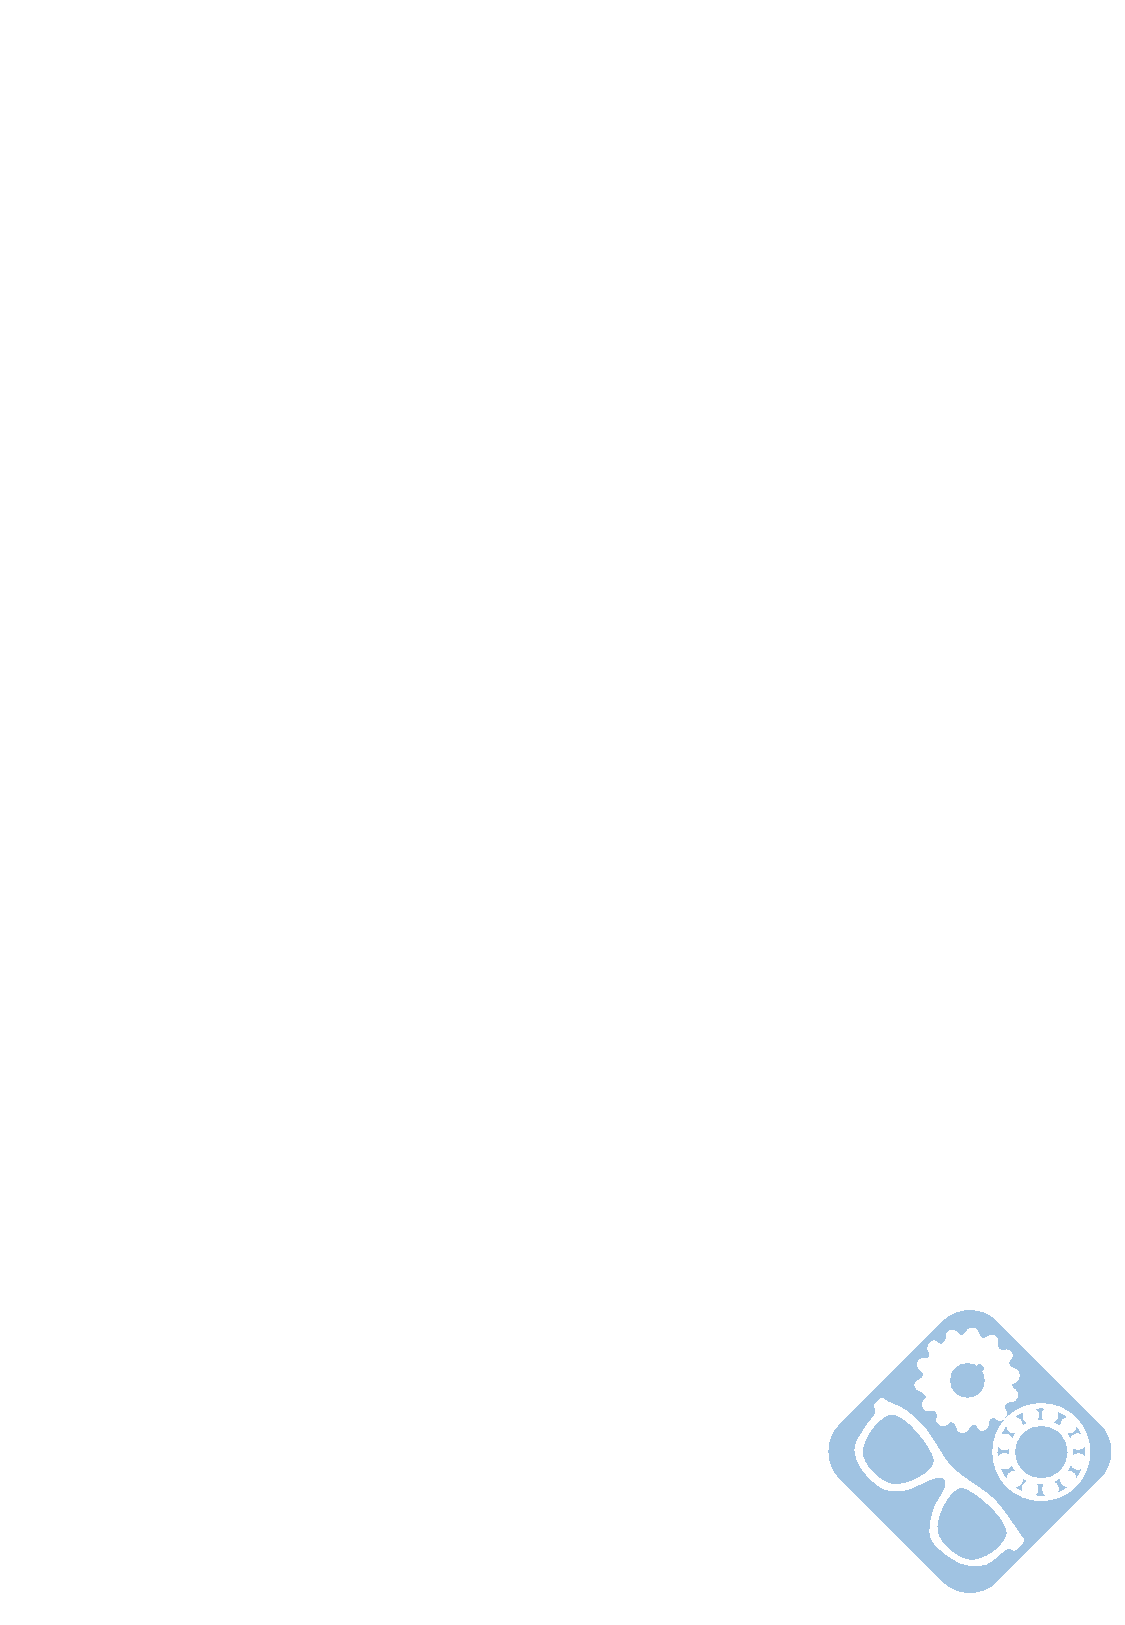
\includegraphics[width=\paperwidth,height=\paperheight,%
keepaspectratio]{../../img/fond4}%
\end{center}
\vfill
}}}

\begin{document}

\pagestyle{empty}

\AddToShipoutPicture*{\BackgroundPic}


\includegraphics[width=2cm]{../../img/logo}

\Huge{DS \num\ - \sujet}

\vspace{1cm}

\ifdef{\prive}{\begin{center}\colorbox{danger}{\Huge{Avec Correction}}\end{center}}{}

\begin{center}
\centering\huge{PTSI}
\end{center}

\vspace{2cm}


\begin{center}
\centering\Large{\jour}
\end{center}

\vspace{2cm}

\normalsize

\tableofcontents

\newpage

\AddToShipoutPicture{\BackgroundPicdeux}

\pagestyle{fancy}

\begin{center}
\Huge \sujet
\end{center}


\normalsize

\textbf{Notations et informations à respecter:}

\begin{itemize}
 \item Pour écrire un torseur cinématique d'un mouvement de $i/j$, au point $P$, dans le repère $R_0$, vous devrez utiliser uniquement la notation imposée suivante: 

$\left\{V_{i/j}\right\}=\left\{
\begin{matrix}
 \omega x_{ij} & Vx_{P,ij} \\
 \omega y_{ij} & Vy_{P,ij} \\
 \omega z_{ij} & Vz_{P,ij} 
\end{matrix}
\right \}_{P,R_0}=\left \{
\begin{matrix}
 \overrightarrow{\Omega_{i/j}} \\ 
 \overrightarrow{V_{P,i/j}} 
\end{matrix}
\right\}_P$
(l'écriture peut être en ligne ou en colonne)

 \item Pour écrire un torseur d'action mécanique transmissible par une liaison de $i\rightarrow j$, au point $P$, dans le repère $R_0$, vous devrez utiliser uniquement la notation imposée suivante: 

$\left\{T_{i\rightarrow j}\right\}=\left\{
\begin{matrix}
 X_{ij} & {L }_{P,ij} \\
 Y_{ij} & {M }_{P,ij} \\
 Z_{ij} & {N }_{P,ij} 
\end{matrix}
\right \}_{P,R_0}=\left \{
\begin{matrix}
 \overrightarrow{R_{i\rightarrow j}} \\ 
 \overrightarrow{M_{P,i\rightarrow j}} 
\end{matrix}
\right\}_P$
(l'écriture peut être en ligne ou en colonne)

 \item Tous vos résultats seront justifiés.
 \item Vous devrez écrire au stylo, pas au critérium, sinon votre copie ne sera pas corrigée.
 \item Une attention particulière sera apportée au soin de votre copie.
\end{itemize}

\newpage

\begin{center}
\Huge Portes de tramway
\end{center}

\normalsize

\section{Présentation de l'étude (30 min)}

\begin{figure}[!h]
\begin{minipage}{0.6\linewidth}
Les grandes métropoles répondent au problème du déplacement des populations par le développement des transports en commun. Dans ce contexte, il est possible d'augmenter le débit des passagers en augmentant la vitesse de déplacement et en diminuant les temps d'arrêt aux gares. Ce dernier point implique que les dispositifs d'accès des passagers aux voitures soient optimisés.

Le support de cette étude est le système d'ouverture et de fermeture des portes de voitures développé par la société FAIVELEY qui équipe des tramways, des métropolitains ou des trains express régionaux. L'étude est limitée à la phase de fermeture d'une porte. Le cahier des charges partiel lors de cette phase est donné sur les figures \ref{fig0} et \ref{fig1}.
\end{minipage}
\hfill
\begin{minipage}{0.35\linewidth}
 \centering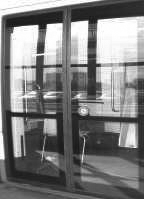
\includegraphics[width=0.8\linewidth]{img/Portes1.png}
\end{minipage}
\end{figure}

\begin{figure}[!h]
 \centering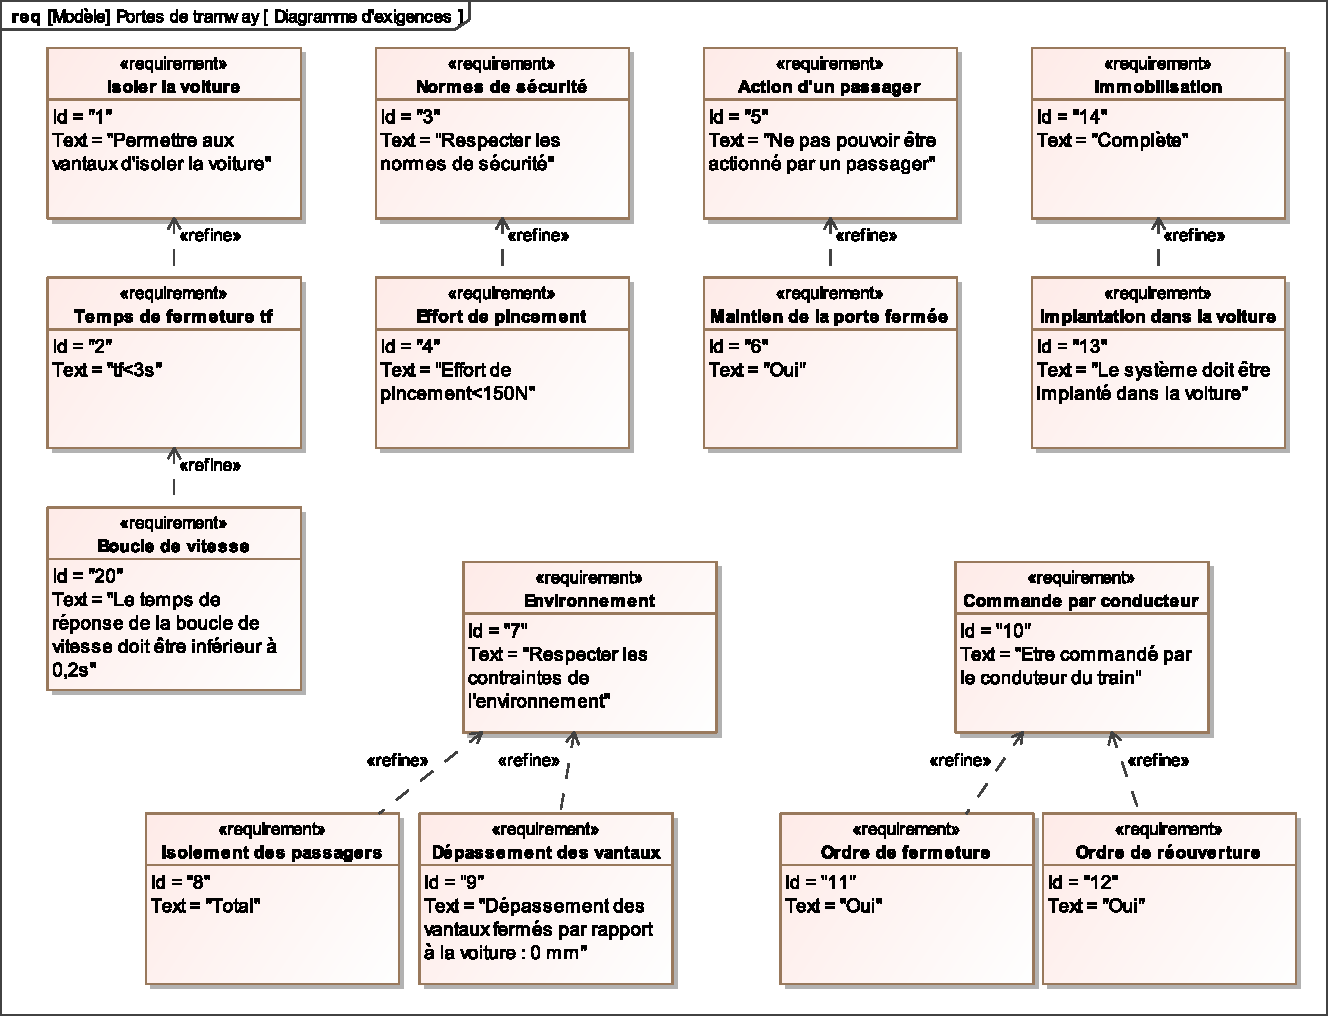
\includegraphics[width=\linewidth]{img/exigences}
 \caption{Diagramme d'exigences}
 \label{fig0}
\end{figure}


%\begin{table}[!h]
% \begin{tabular}{|m{7cm}|m{6cm}|m{2cm}|}
%\hline
%Fonction & Critères & Niveaux \\
%\hline
%$FP_1$: Permettre aux vantaux d'isoler la voiture & Temps de fermeture $t_f$ & $\leq 3s$ \\
%\hline
%$FC_1$: Respecter les normes de sécurité & Effort de pincement & $\leq 150N$ \\
%\hline
%$FC_2$: Ne pas pouvoir être actionné par un passager & Maintien de la porte fermée & Oui \\
%\hline
%$FC_3$: Respecter les contraintes de l'environnement & Isolement des passagers & Total \\
%\hline
%& Dépassement des vantaux fermés par rapport à la voiture & $0mm$ \\
%\hline
%$FC_4$: Etre commandé par le conducteur de train & Ordre de fermeture & Oui \\
%\hline
%& Ordre de réouverture & Oui \\
%\hline
%$FC_5$: Être implanté sur la voiture & Immobilisation & Complète\\
%\hline
% \end{tabular}
%\end{table}

\begin{figure}[!h]
 \centering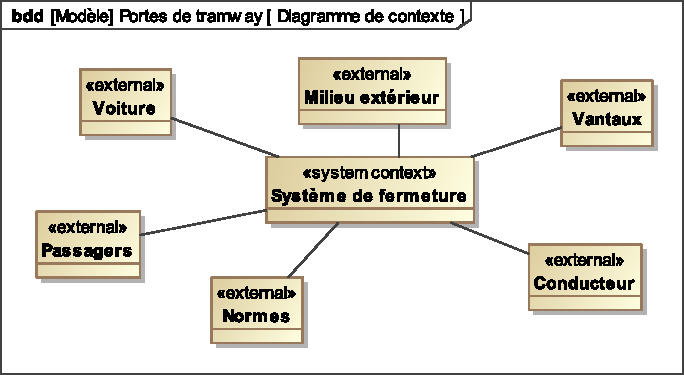
\includegraphics[width=0.8\linewidth]{img/contexte}
 \caption{Diagramme de contexte}
 \label{fig1}
\end{figure}

\newpage

Chacune des portes est constituée de deux vantaux qui, ouverts, sont immobilisés le long de la voiture pour dégager la totalité de l'ouverture de la voiture.

\begin{figure}[!h]
 \centering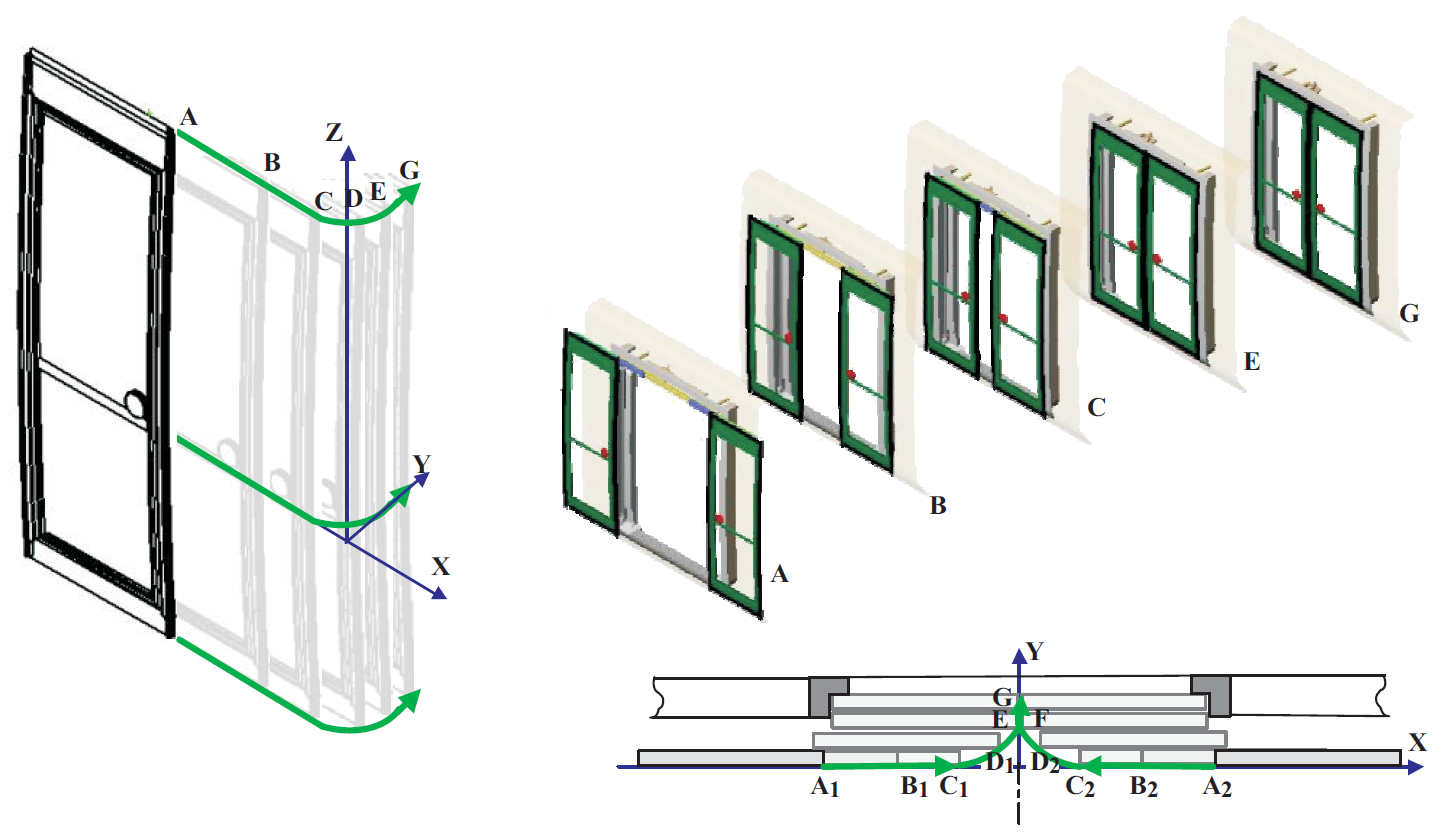
\includegraphics[width=0.8\linewidth]{img/Portes3.png}
 \caption{Phase de fermeture}
 \label{fig2}
\end{figure}

La phase de fermeture peut être décomposée en trois étapes dont quelques positions d'un point, appartenant au vantail le long de sa trajectoire par rapport à la voiture, sont données sur la figure \ref{fig2} :
\begin{itemize}
 \item de A à C: étape de coulissement ; les vantaux coulissent parallèlement à la voiture et l'écartement passe de $1300mm$ à $200mm$,
 \item De C à E: étape de louvoiement ; les vantaux continuent de se rapprocher jusqu'au contact et rentrent dans l'ouverture de la porte pour ne plus dépasser à l'extérieur.
 \item De E à G: étape de verrouillage ; les vantaux se déplacent légèrement pour comprimer les joints d'étanchéité et se verrouillent.
\end{itemize}

Le système est principalement constitué des composants identifiés sur la figure \ref{fig3}. La poutre de fermeture est guidée dans son mouvement de translation suivant $\overrightarrow{y}$ par les deux boîtes à galets implantées sur la voiture.

Elle supporte le mécanisme d'entraînement constitué d'un actionneur unique, le moto réducteur, d'éléments de transmission et de la courroie crantée. Elle supporte également les glissières à billes qui assurent le guidage en translation des vantaux lorsqu'ils sont entraînés par la courroie.

\begin{figure}[!h]
 \centering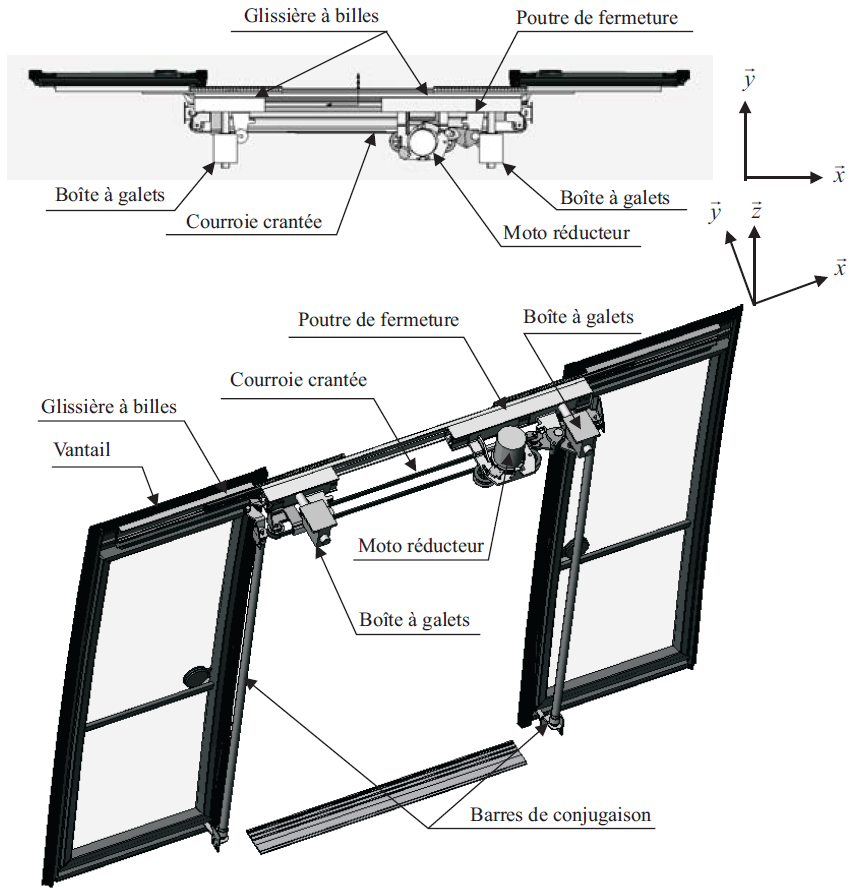
\includegraphics[width=0.8\linewidth]{img/Portes4.png}
 \caption{Description du système}
 \label{fig3}
\end{figure}

\paragraph{Question 1:} Compléter le diagramme d'exigences donné sur le document réponse 1 en précisant les fonctions techniques réalisées par les composants. Pour la suite de l'étude, la modélisation du système retenue est donnée sur le schéma de la figure \ref{fig4}.

Cette modélisation permet d'appréhender la fonction des éléments de transmission tels que la barre de conjugaison, la bielle de verrouillage ou le basculeur. La modélisation fait apparaître également les différentes liaisons du rotor et du stator du motoréducteur.

\begin{figure}[!h]
 \centering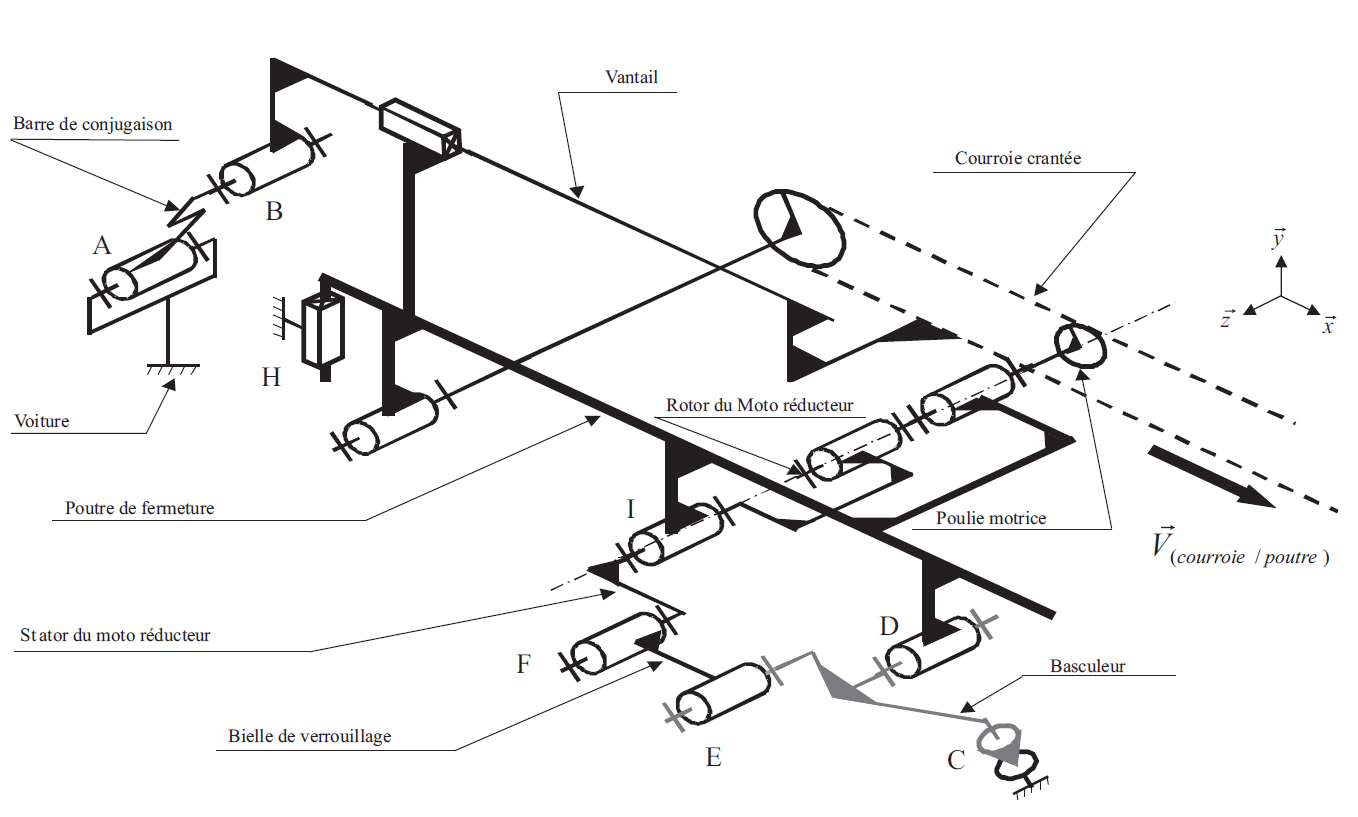
\includegraphics[width=0.8\linewidth]{img/Portes5.png}
 \caption{Schéma cinématique}
 \label{fig4}
\end{figure}

\newpage

Pendant l'étape de coulissement, figure \ref{fig5}, la poutre de fermeture est immobile par rapport à la voiture. Le motoréducteur entraîne la courroie crantée qui elle-même entraîne les vantaux.

\begin{figure}[!h]
 \centering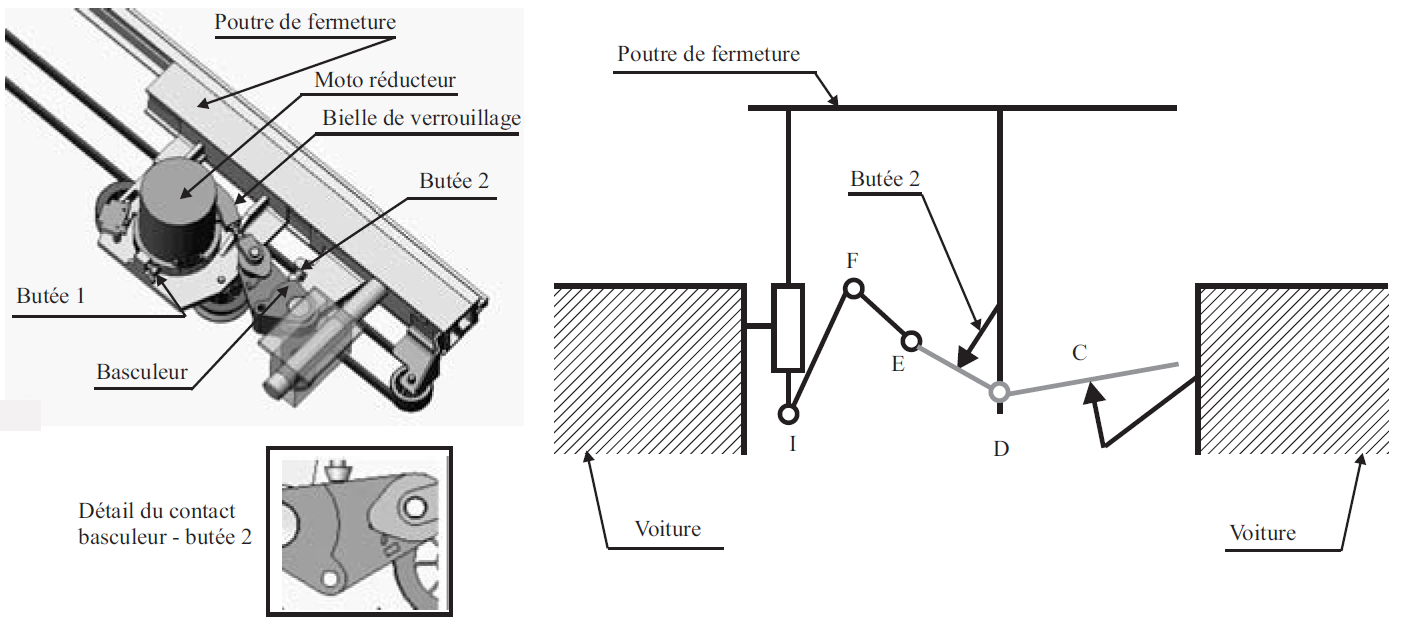
\includegraphics[width=0.7\linewidth]{img/Portes6.png}
 \caption{Étape de coulissement}
 \label{fig5}
\end{figure}

\begin{figure}[!h]
\begin{minipage}{0.48\linewidth}
Pendant cette étape, le galet installé à l'extrémité supérieure de la barre de conjugaison, figure \ref{fig6}, roule dans la rainure du vantail.
\end{minipage}
\hfill
\begin{minipage}{0.5\linewidth}
 \centering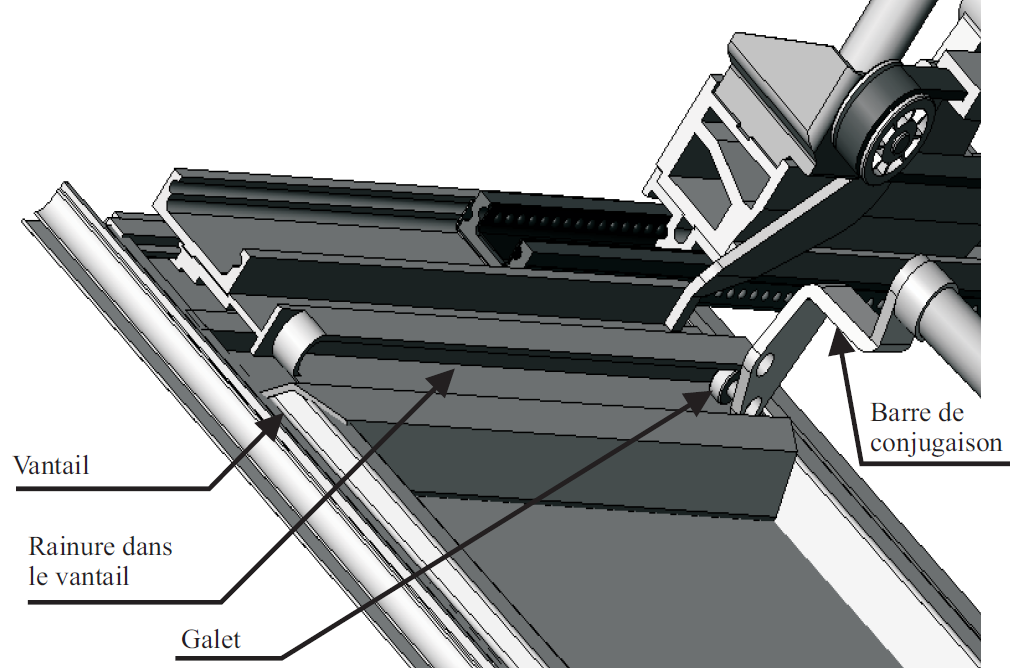
\includegraphics[width=0.8\linewidth]{img/Portes7.png}
 \caption{Barre de conjugaison}
 \label{fig6}
\end{minipage}
\end{figure}

\begin{figure}[!h]
\begin{minipage}{0.6\linewidth}
L'étape de louvoiement, figure \ref{fig7}, commence lorsque le galet arrive en butée à l'extrémité de la rainure. Pendant cette étape, les vantaux continuent de se rapprocher et le galet entraîne en rotation la barre de conjugaison qui elle-même entraîne la translation de la poutre de fermeture.

La translation de la poutre de fermeture suivant la direction $\overrightarrow{y}$ provoque la rotation du basculeur $EDC$ (en liaison pivot d'axe $(D,\overrightarrow{z})$ avec la poutre de fermeture), par l'intermédiaire d'une liaison ponctuelle (ou sphère-plan) entre la voiture et le basculeur au point $C$.
\end{minipage}
\hfill
\begin{minipage}{0.35\linewidth}
 \centering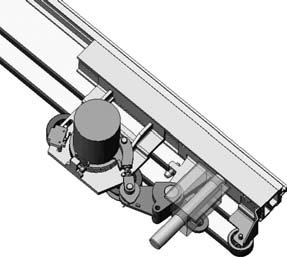
\includegraphics[width=0.8\linewidth]{img/Portes8.png}
 \caption{Phase de louvoiement}
 \label{fig7}
 \end{minipage}
\end{figure}

Le basculeur, par l'intermédiaire de la bielle de verrouillage $EF$ va libérer le \og stator \fg du moto réducteur en liaison pivot d'axe $(I,\overrightarrow{z})$ avec la poutre de fermeture. Ainsi, pendant cette étape, la poulie motrice et le \og stator \fg $IF$ du moto réducteur tournent par rapport à la poutre de fermeture.

Pendant l'étape de verrouillage (de E à G), le mouvement de rotation du \og stator \fg va permettre le verrouillage de la porte. La figure \ref{fig8} montre le système pendant cette étape et le schéma du système verrouillé.

\begin{figure}[!h]
 \centering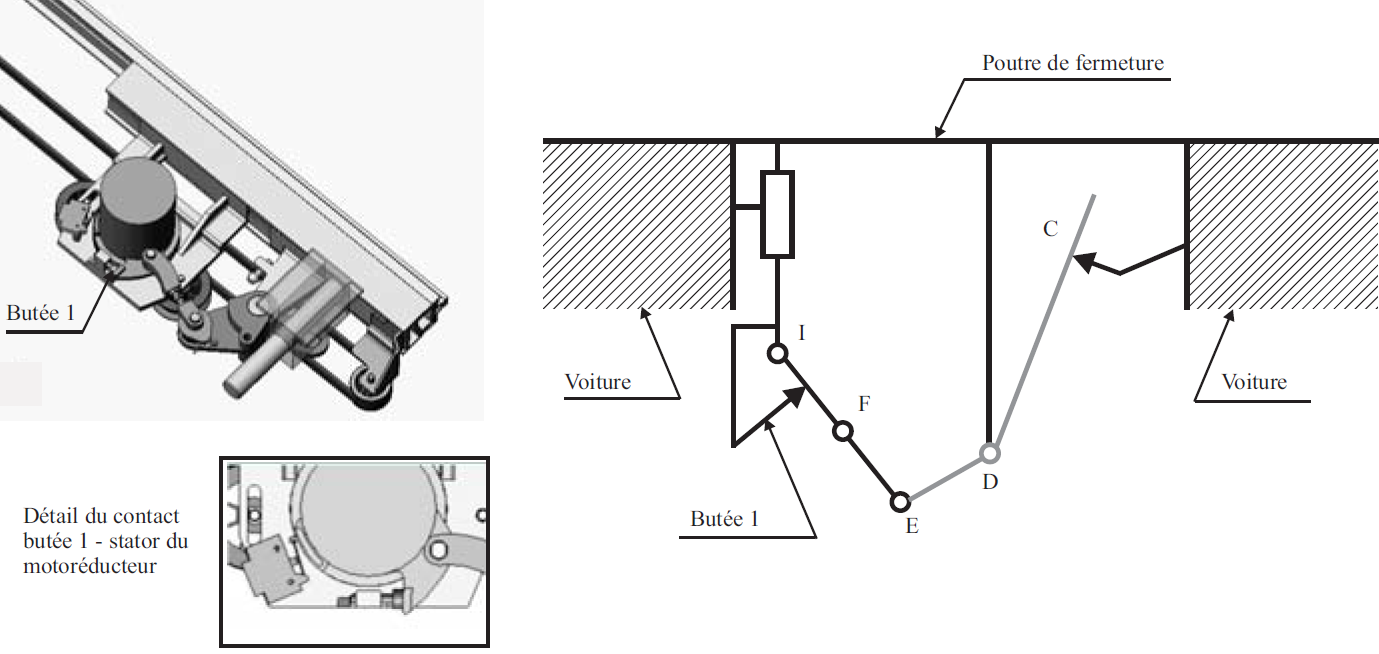
\includegraphics[width=0.8\linewidth]{img/Portes9.png}
 \caption{Étape verrouillée}
 \label{fig8}
\end{figure}

Dans les transports en commun, la sécurité des personnes transportées constitue un souci prioritaire, préalable à celui de la rapidité et du confort. L'objet de ce sujet est de valider la conformité aux normes de sécurité, pour le temps de fermeture des vantaux attendu.

\newpage

\section{Étude partielle de la phase de fermeture (30min)}

\subsection{Étude de l'étape de coulissement des vantaux}

\begin{figure}[!h]
\begin{minipage}{0.6\linewidth}
La figure \ref{fig9} est une photo du dispositif d'entraînement de la courroie crantée sur laquelle les vantaux sont fixés pour être entraînés.
\paragraph{Question 2:} Compléter le schéma du document réponse 2, que vous rendrez avec votre copie, en proposant des modèles de liaisons entre les vantaux et et la courroie crantée ; et dans les zones et entre
les vantaux et et la poutre de fermeture.
\end{minipage}
\hfill
\begin{minipage}{0.35\linewidth}
 \centering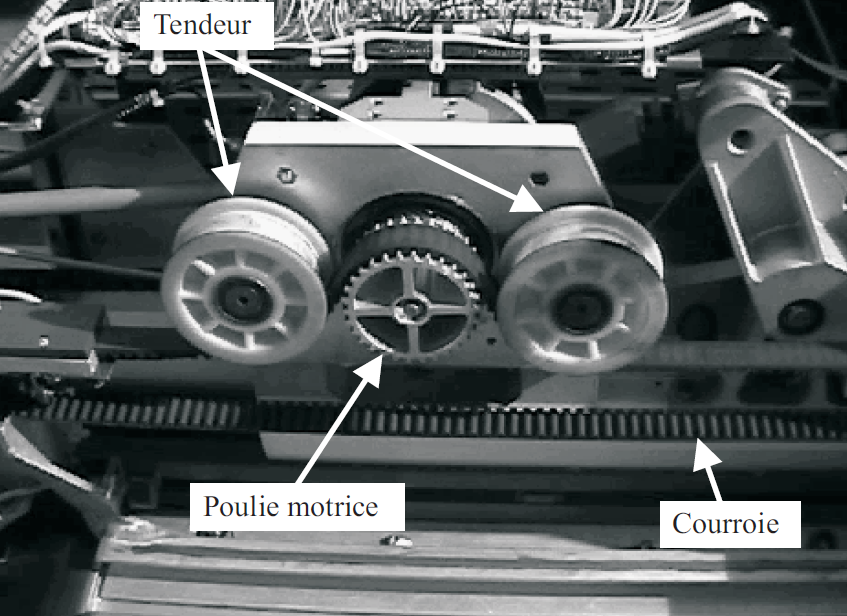
\includegraphics[width=0.8\linewidth]{img/Portes10.png}
 \caption{Poulies-courroie}
 \label{fig9}
 \end{minipage}
\end{figure}

\subsection{Étude de la poutre de fermeture}

\subsubsection{Étude du guidage de la poutre de fermeture}

\begin{figure}[!h]
\begin{minipage}{0.6\linewidth}
Pour réaliser la fonction $FC_3$, les vantaux doivent avoir un mouvement de translation de direction $\overrightarrow{y}$ par rapport à la voiture, figure \ref{fig2}. Ce mouvement est assuré par le guidage de la
poutre de fermeture grâce à deux boîtes à galets placées aux points $H$ et $J$ de la figure \ref{fig10} qui donne le modèle retenu pour chacune d'elles.
\end{minipage}
\hfill
\begin{minipage}{0.35\linewidth}
 \centering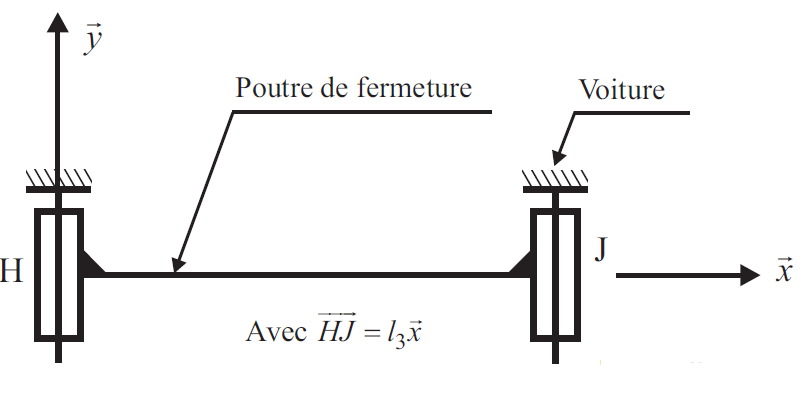
\includegraphics[width=\linewidth]{img/Portes11.png}
 \caption{Poutre de fermeture}
 \label{fig10}
 \end{minipage}
\end{figure}

L'objet de cette partie est de trouver la liaison équivalente à l'association de ces deux liaisons.

\paragraph{Question 3:} Déterminer le degré d'hyperstatisme de ce modèle. En déduire les contraintes géométriques à satisfaire lors de la réalisation,

\paragraph{Question 4:} Proposer une liaison élémentaire cinématiquement équivalente à ces deux liaisons et exprimer son torseur cinématique caractéristique,

\paragraph{Question 5:} Proposer et justifier un modèle pour la liaison élémentaire au point J qui rende la liaison résultante isostatique.

\subsubsection{Étude du système de mise en mouvement de la poutre de fermeture}

Le document réponse 3 représente les schémas cinématiques du mécanisme pour les trois étapes de fonctionnement.

\begin{figure}[!h]
 \centering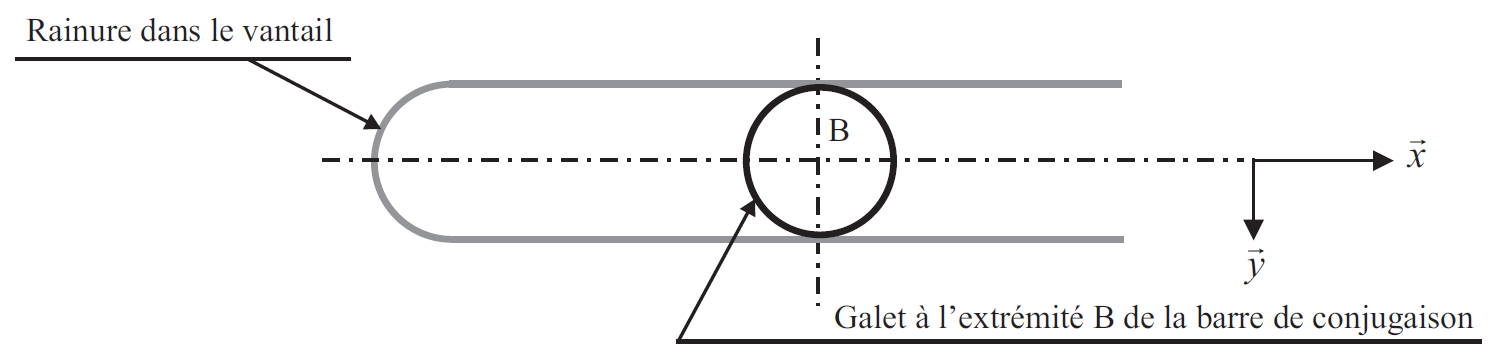
\includegraphics[width=0.8\linewidth]{img/Portes12.png}
 \caption{Système de mise en mouvement}
 \label{fig11}
\end{figure}

\paragraph{Question 6:} Compléter les schémas du document réponse 3 qui sera rendu avec la copie, en représentant la barre de conjugaison et en indiquant pour chaque étape la liaison équivalente entre la barre de conjugaison et le vantail.

Remarques :
\begin{itemize}
 \item Pour la phase coulissement, la barre de conjugaison est parallèle à l'axe,
 \item Le galet de forme cylindrique est en liaison rotule (ou sphérique) avec la barre de conjugaison.
\end{itemize}

\section{Étude de la phase de verrouillage (1h)}

\begin{figure}[!h]
\begin{minipage}{0.49\linewidth}
Le système de verrouillage doit maintenir la porte fermée sous l'action des passagers et des actions dues aux différences de pressions induites par le système de climatisation.

La fermeture de la porte doit être douce afin de ne pas bousculer les passagers lors des périodes de forte affluence. Le modèle du dispositif retenu est donné sur la figure \ref{fig12}.
\end{minipage}
\hfill
\begin{minipage}{0.49\linewidth}
 \centering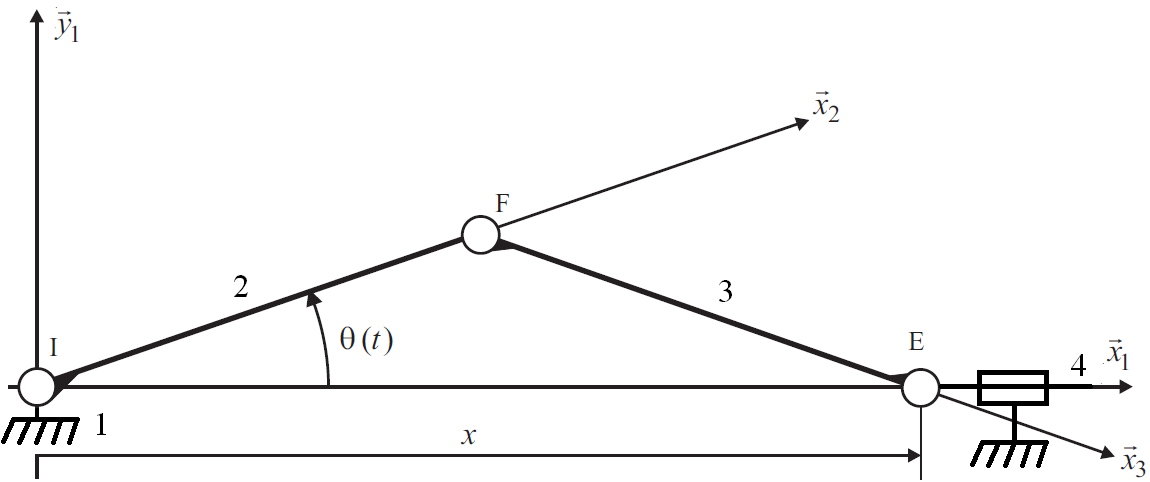
\includegraphics[width=\linewidth]{img/Portes13.png}
 \caption{Modèle du dispositif}
 \label{fig12}
 \end{minipage}
\end{figure}

Soit le repère $R_1(I,\overrightarrow{x_1},\overrightarrow{y_1},\overrightarrow{z_1})$ tel que $\overrightarrow{x_1}$ soit colinéaire à $\overrightarrow{IE}$ dans toutes les configurations de la bielle de verrouillage $FE$ et du bras $IF$ lié au \og stator \fg du motoréducteur. Les notations retenues sont celles définies sur la figure \ref{fig4}, les liaisons entre la bielle de verrouillage et le basculeur et entre le stator et la poutre de fermeture sont respectivement une liaison pivot d'axe $(E,\overrightarrow{z_1})$ et une liaison pivot d'axe $(I,\overrightarrow{z_1})$.

$(I,\overrightarrow{x_2})$ est lié au stator et tel que $(\overrightarrow{x_1},\overrightarrow{x_2})=\theta(t)$,

$(F,\overrightarrow{x_3})$ est lié à la bielle de verrouillage et tel que $\overrightarrow{x_3}$ soit colinéaire à $\overrightarrow{FE}$.

Pendant la phase de verrouillage, $\theta(t)$ varie quand le stator du moto réducteur tourne par rapport à la poutre de fermeture. La vitesse angulaire sera notée $\dot{\theta}(t)$, $\overrightarrow{IF}=l_1.\overrightarrow{x_2}$ et $\overrightarrow{FE}=l_2.\overrightarrow{x_3}$, par construction $l_1\neq l_2$.


\paragraph{Question 7:} Exprimer $x(t)$ en fonction de $l_1$, $l_2$ et $\theta(t)$ sous la forme $x(t)=\lambda_1(t).l_1+l_2.\sqrt{1-r.\lambda_2(t)}$,

\paragraph{Question 8:} Montrer qu'il existe une loi de fermeture cinématique entre les pièces de la figure \ref{fig12} .

\paragraph{Question 9:} Écrire les torseurs de chacune des liaisons présentes sur la figure \ref{fig12}.

\paragraph{Question 10:} Écrire la vitesse du point E $V_{E\in 4/1}$ en fonction de la vitesse de rotation de $2/1$ et des paramètres géométriques du système.

\section{Étude de la commande de la chaîne de motorisation (1h15)}

La figure \ref{asserv1} représente l'organisation fonctionnelle de la structure d'asservissement. La consigne de vitesse dépend de la position de la porte mais pour des raisons pratiques la réalisation de ces deux boucles est effectuée à partir des mesures de la position et de la vitesse angulaire de l'arbre moteur.

\begin{figure}[!h]
 \centering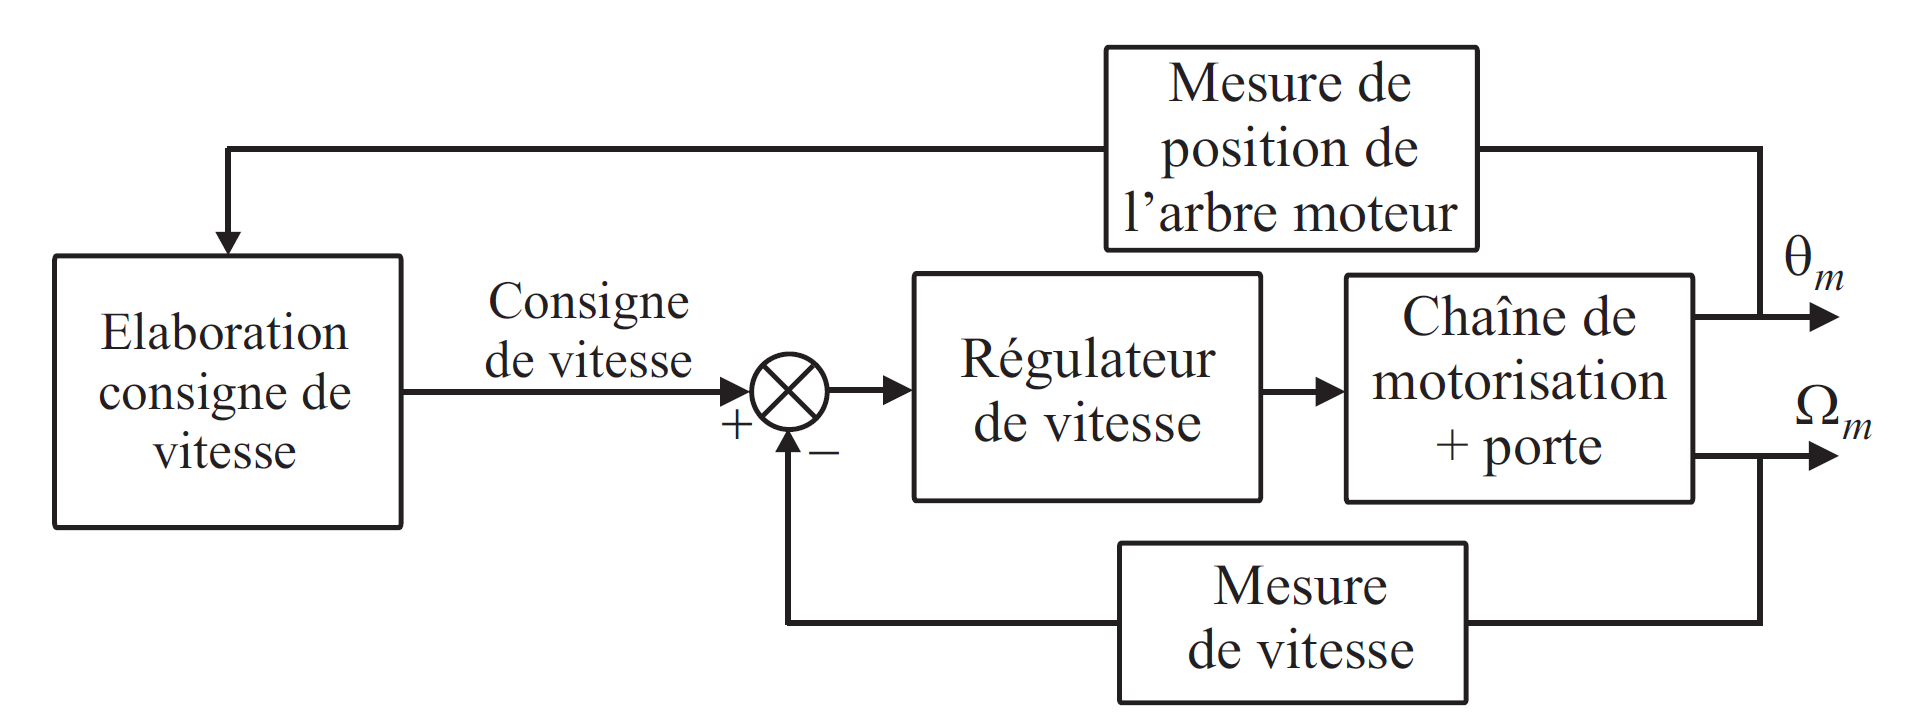
\includegraphics[width=0.8\linewidth]{img/asserv1}
 \caption{Structure de commande de la chaîne de motorisation}
 \label{asserv1}
\end{figure}

Cette partie a comme objectif d'une part l'étude de la chaîne d'asservissement de
vitesse, d'autre part la vérification du cahier des charges pour la structure et la
loi de commande retenues. L'élaboration de la consigne de vitesse à partir de la
boucle de position est hors du cadre de ce sujet.

\subsection{Étude du régulateur de la boucle de vitesse}

\begin{figure}[!h]
\begin{minipage}{0.49\linewidth}
La chaîne de régulation de vitesse est décrite par le schéma bloc de la figure \ref{asserv2} où la fonction de transfert $H_3(p)$ représente la chaîne de mesure de vitesse comportant un filtre du 1er ordre, de constante de temps $\tau_f=10ms$, permettant de limiter l'impact des bruits de mesure et $G$ est le gain de l'amplificateur de puissance alimentant le moteur. \\
Dans la suite la perturbation $F_1$ sera considérée comme nulle.
\end{minipage}
\hfill
\begin{minipage}{0.49\linewidth}
 \centering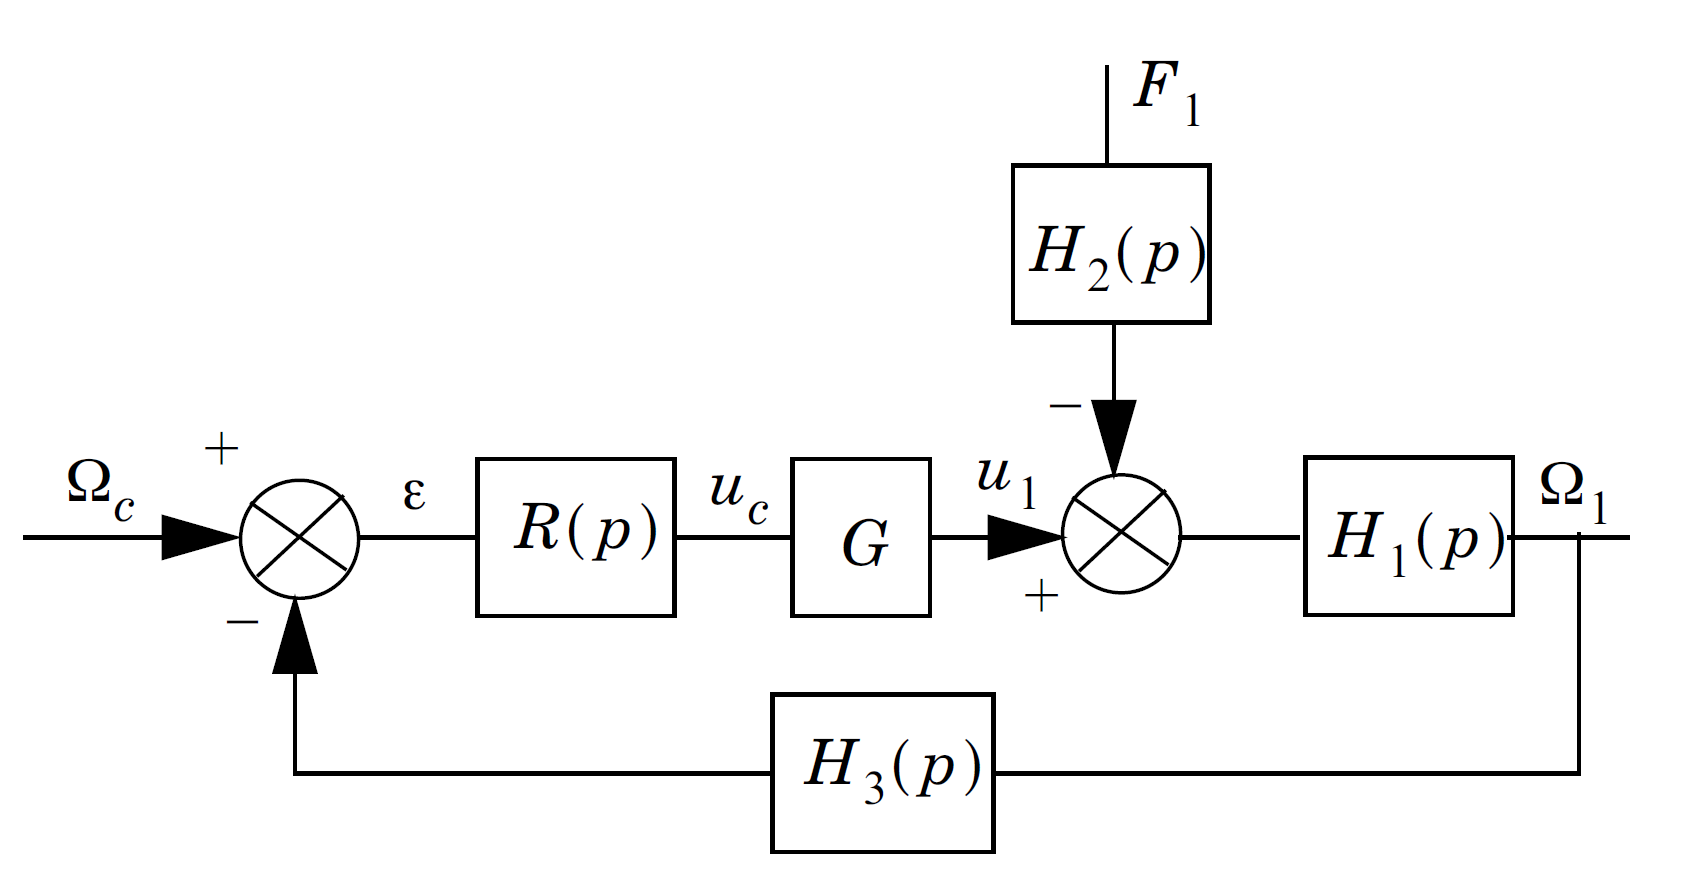
\includegraphics[width=\linewidth]{img/asserv2}
 \caption{Schéma bloc de la boucle de régulation de vitesse}
 \label{asserv2}
 \end{minipage}
\end{figure}

\subsubsection{Première correction}

On choisit d'adopter pour cette chaîne un régulateur de type proportionnel (P) dont la fonction de transfert est $R(p)=K_r=1$.

On adopte les modèles de commande simplifiés suivants:

$H_1(p)=\frac{10}{p}$, $H_2(p)=0,05$, $H_3(p)=\frac{0,1}{1+0,01.p}$, $G=10$.

\paragraph{Question 11:} Déterminer la Fonction de Transfert en Boucle Fermée $H(p)=\frac{\Omega_1(p)}{\Omega_c(p)}$, la mettre sous la forme canonique. Donner sa classe et son ordre.

\paragraph{Question 12:} Montrer que cette fonction peut s'écrire sous la forme d'un premier ordre. Donner ses caractéristiques.

\paragraph{Question 13:} Déterminer la loi de sortie temporelle $\omega_1(t)$ lorsque l'entrée est un échelon unitaire.

\paragraph{Question 14:} Tracer cette réponse temporelle sur le document réponse.

\paragraph{Question 15:} Donner alors son temps de réponse à 5\%, le système ainsi configuré répond-il au cahier des charges ?

\subsubsection{Seconde correction}

Dans la suite, on choisit d'adopter pour cette chaîne un régulateur de type proportionnel-intégral (PI) dont la fonction de transfert est :
$R(p)=K_r.\left(1+\frac{1}{T_i.p}\right)$, avec $K_r=1$ et $T_i=0,1s$.

\paragraph{Question 16:}

Déterminer la Fonction de Transfert en Boucle Fermée $H(p)=\frac{\Omega_1(p)}{\Omega_c(p)}$, la mettre sous la forme canonique. Donner sa classe et son ordre.

~\

Le tracé de Bode de cette fonction est donné sur la figure \ref{asserv3}.

\begin{figure}[!h]
 \centering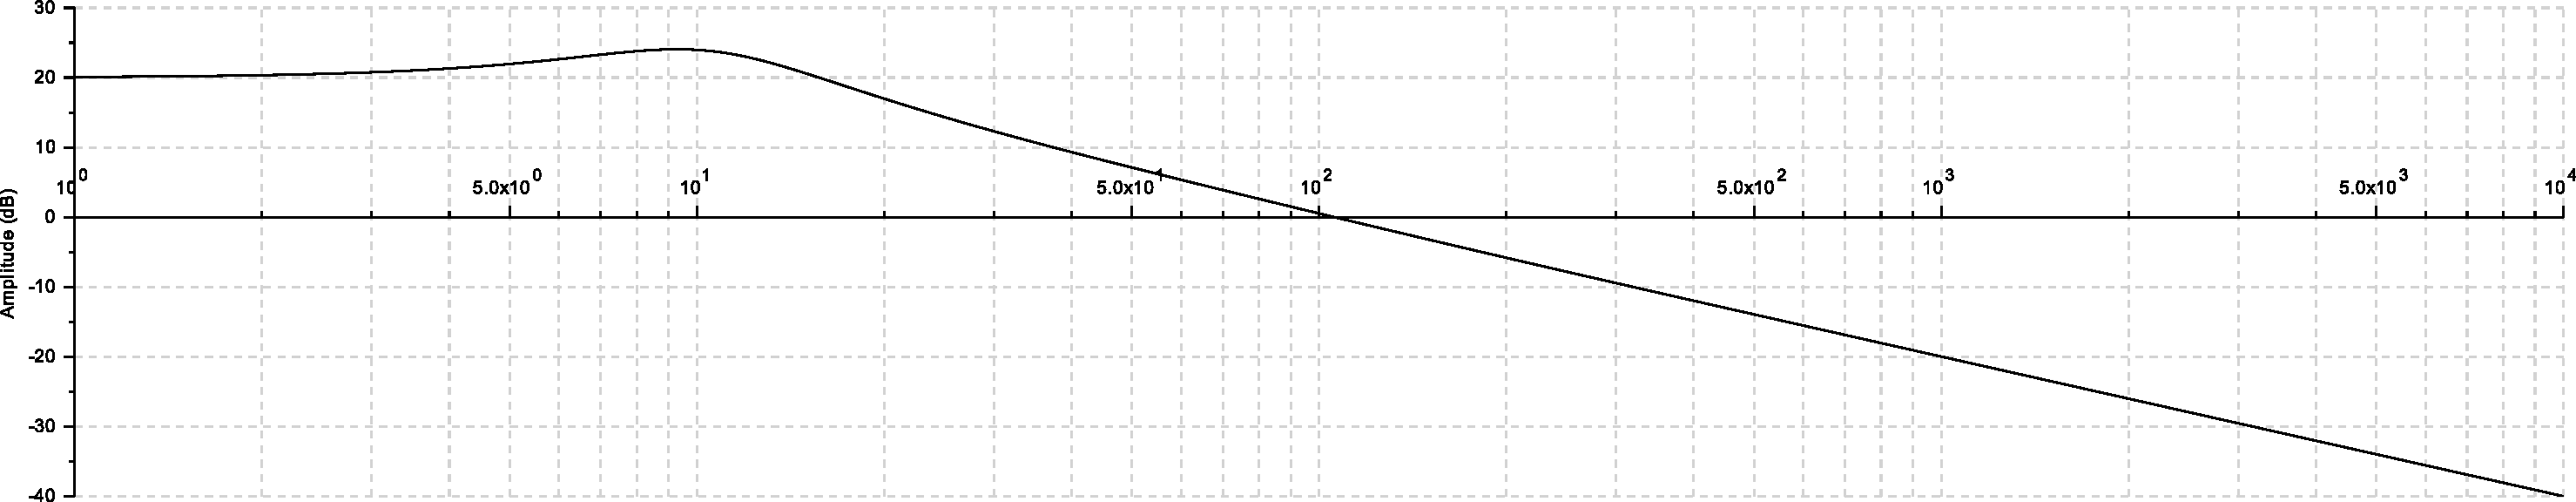
\includegraphics[width=\linewidth]{img/bode}
 \caption{Tracé de Bode de la fonction de transfert en boucle fermée $H(p)$}
 \label{asserv3}
\end{figure}

\paragraph{Question 17:}

Tracer pour l'intervalle $[10^2,+\infty[$ la fonction de transfert du premier ordre la plus proche du tracé de $H(p)$. Déterminer ses caractéristiques.

\paragraph{Question 18:}

Tracer pour l'intervalle $-]\infty,10^1[$ la fonction de transfert du second ordre la plus proche du tracé de $H(p)$. Déterminer ses caractéristiques.

\newpage

Le tracé de H(p) pour une réponse indicielle est donné sur la figure \ref{asserv4}.

\begin{figure}[!h]
 \centering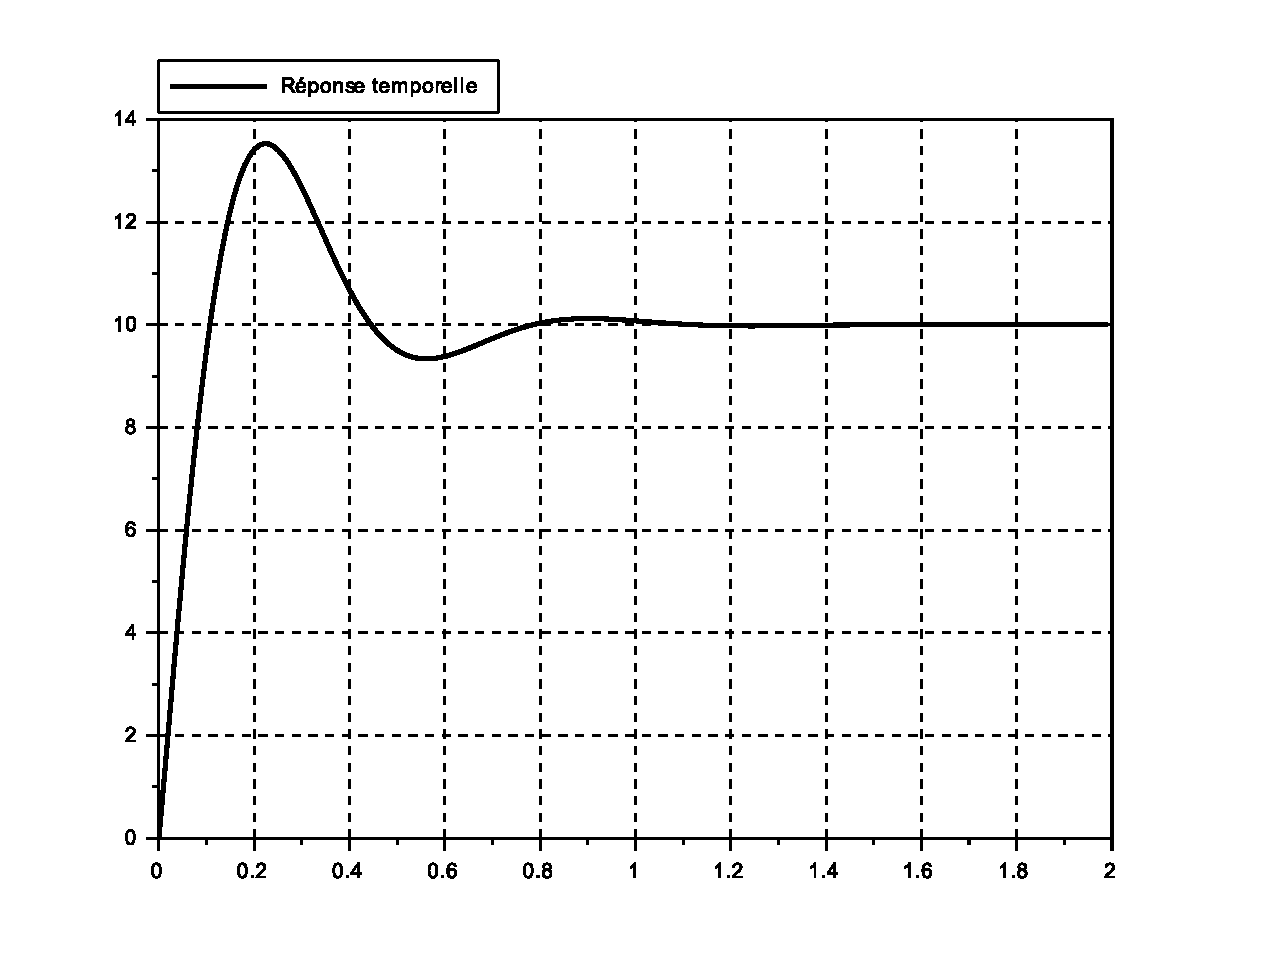
\includegraphics[width=0.6\linewidth]{img/q19}
 \caption{Réponse indicielle de la fonction de transfert en boucle fermée $H(p)$}
 \label{asserv4}
\end{figure}

\paragraph{Question 19:} En assimilant ce tracé à une fonction du second ordre, déterminer ses caractéristiques. On donne $ln(0,35)=-1,05$ et $(\frac{1,05}{\pi})^2=0,11$.


\paragraph{Question 20:} Déterminer le temps de réponse à 5\%, $t_{R5\%}$, du système.

\paragraph{Question 21:} Conclure quant à l'intérêt de la mise en place de cette seconde correction.

\newpage

\section{Étude du système de verrouillage de la porte (45 min)}

Le système de verrouillage de la porte est présenté sur la figure \ref{fig13}

\begin{figure}[!h]
 \centering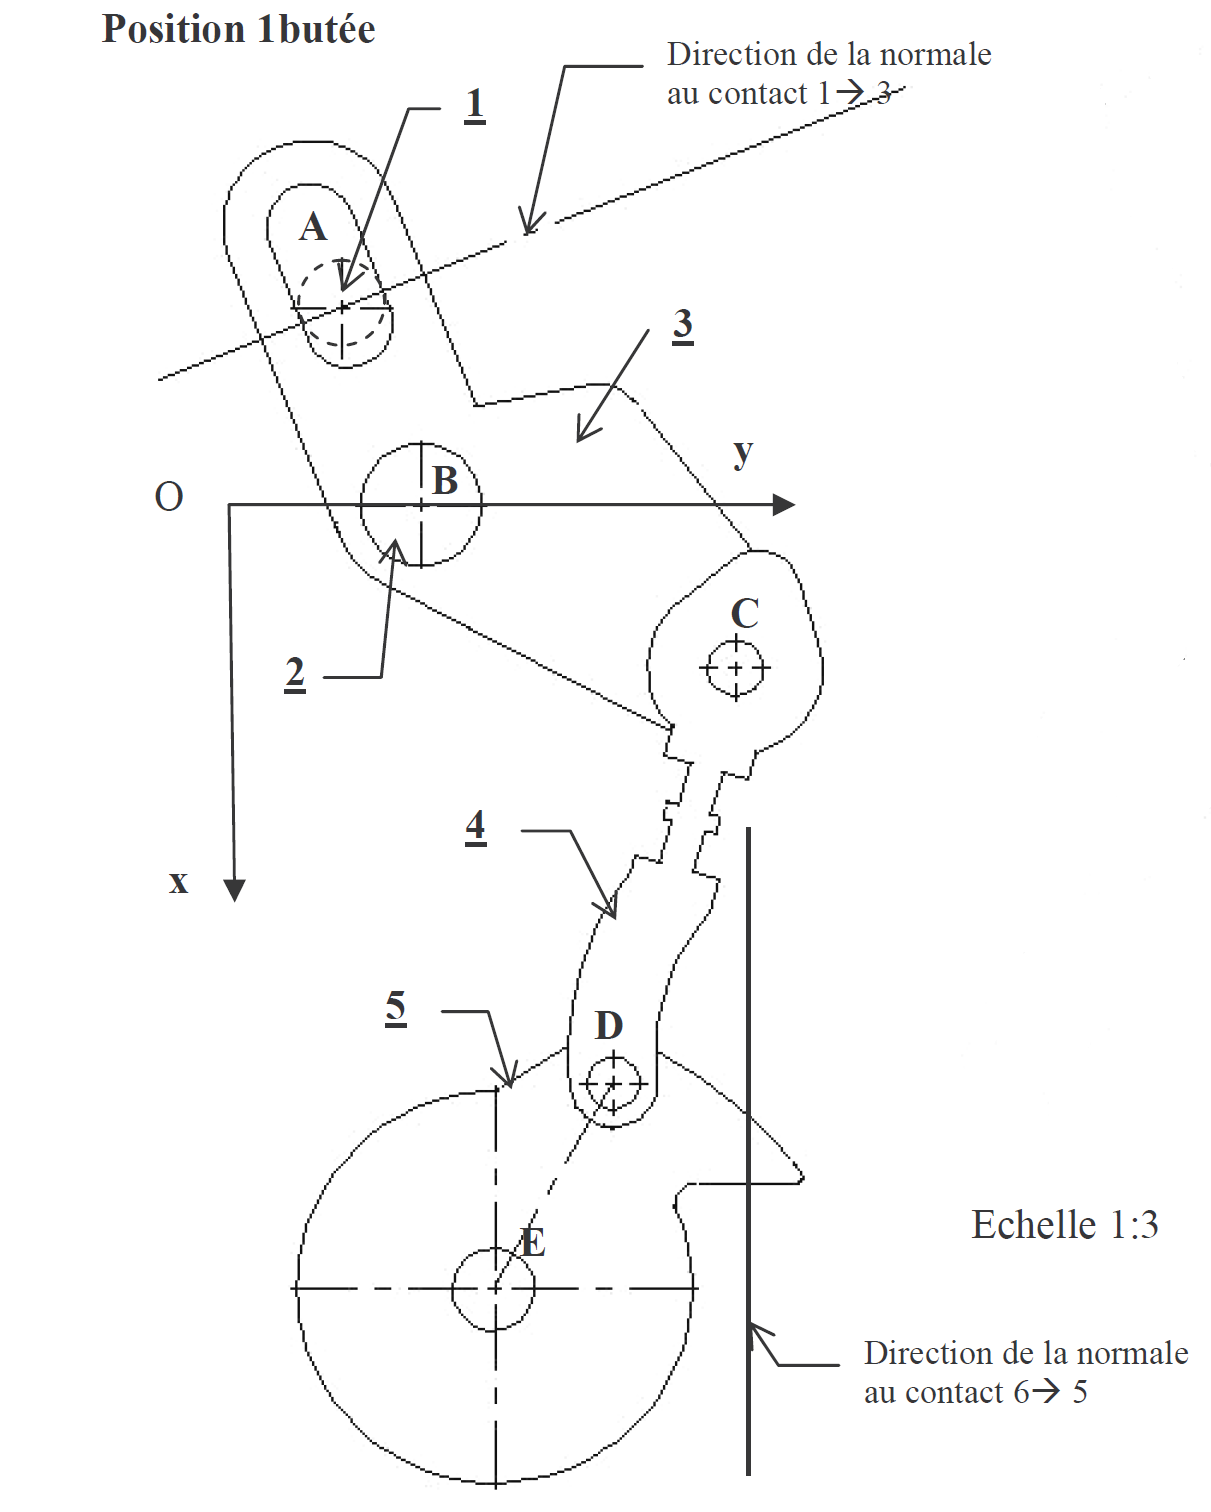
\includegraphics[width=0.7\linewidth]{img/Portes15}
 \caption{Système de verrouillage de la porte}
 \label{fig13}
\end{figure}

La rotation de la pièce 3 autour du point B, sous l'action de la pièce 1 a pour effet d'entrainer en rotation la pièce 5 dans le sens trigonométrique jusqu'à ce que la direction de la normale au contact $6\rightarrow 5$ soit horizontale avec le point D au dessus de E.

\paragraph{Question 22:} Réaliser le schéma cinématique de ce mécanisme.

\paragraph{Question 23:} Représenter, sur le document réponse, ce système en position verrouillée (de façon à ce que la direction de la normale au contact $6\rightarrow 5$ soit horizontale avec le point D au dessus de E).

~\

Le point A se déplace selon la normale au contact $1\rightarrow 3$.

\paragraph{Question 24:} Quelle distance doit-il parcourir afin de verrouiller la porte ?

La pièce 4 est en réalité un assemblage entre deux pièces liées par un assemblage par vis, comme le montre la figure \ref{fig14} Cela permet de pouvoir régler la distance CD au montage du système.

\begin{figure}[!h]
 \centering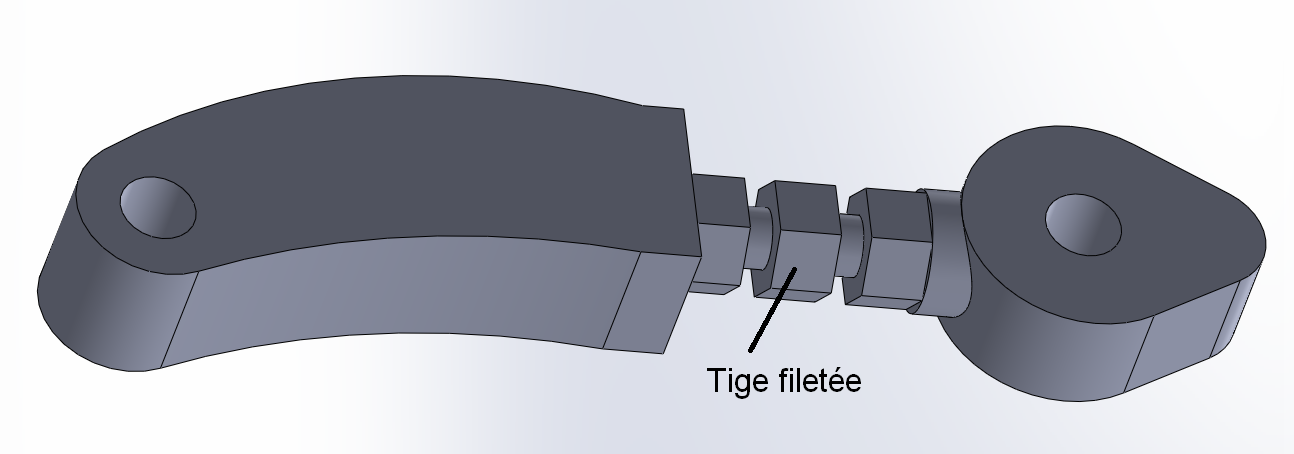
\includegraphics[width=0.7\linewidth]{img/assemblage}
 \caption{Pièce 4}
 \label{fig14}
\end{figure}

La pièce qui relie les deux parties de l'ensemble pièce 4 est une tige filetée des deux côtés avec un écrou encastré au milieu, comme le montre la figure \ref{fig15}.

\begin{figure}[!h]
 \centering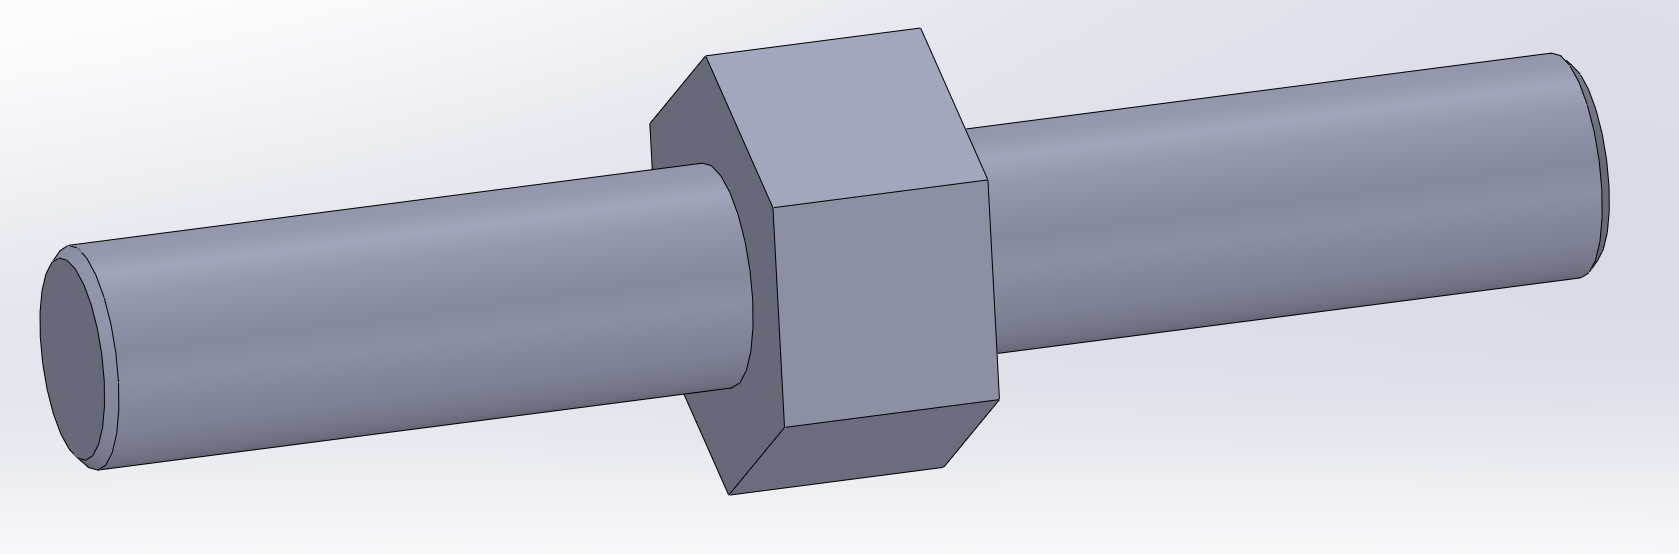
\includegraphics[width=0.6\linewidth]{img/vis}
 \caption{Tige filetée}
 \label{fig15}
\end{figure}

\paragraph{Question 25:} Représenter sur la pièce 4 dans le cadre réservé à cet effet sur la vue en coupe du document réponse.

\paragraph{Question 26:} Quelles caractéristiques doivent avoir les deux filets de chaque côté de l'écrou sur la tige filetée.

\cleardoublepage

\pagestyle{documentreponse}

\section{Document réponse}

\reponse{1}{0}

\begin{center}
 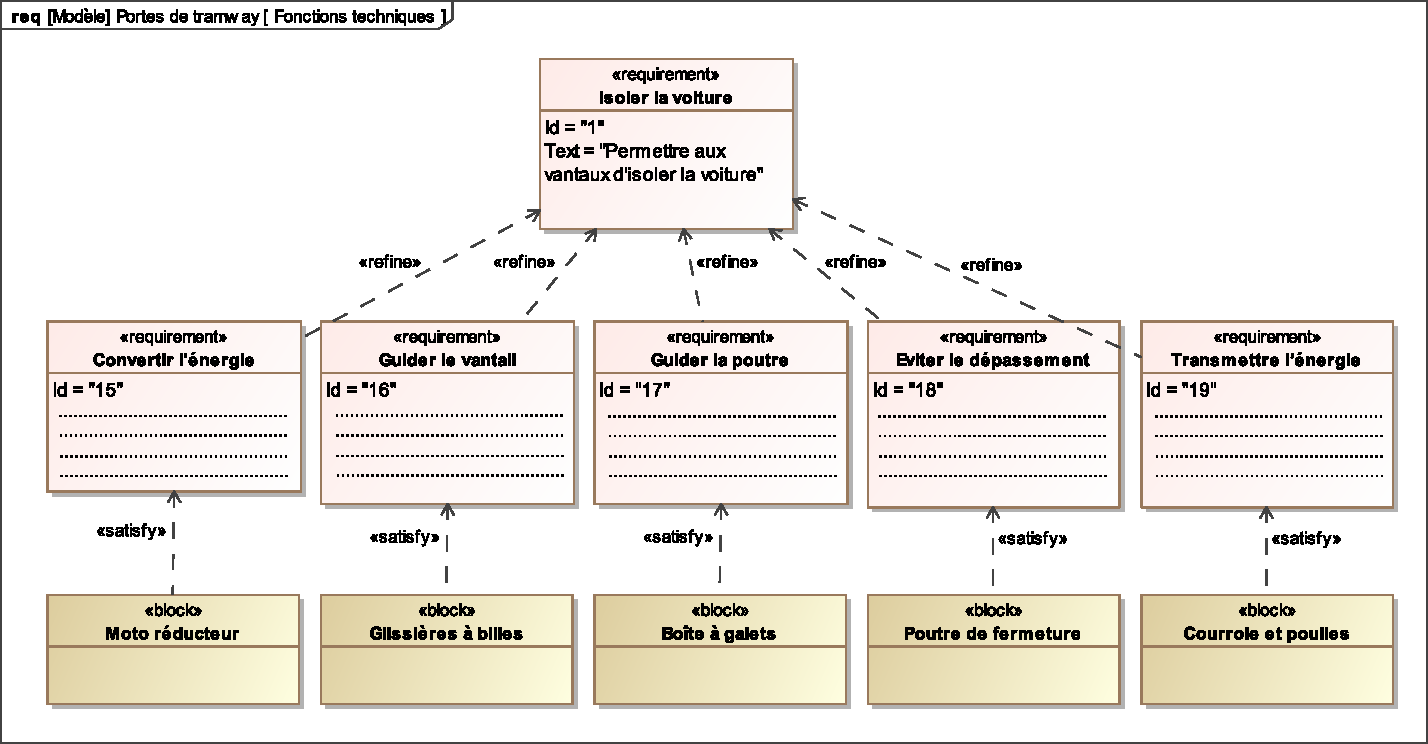
\includegraphics[width=\linewidth]{img/fonctions_techniques}
\end{center}

\reponse{2}{0}

\begin{center}
 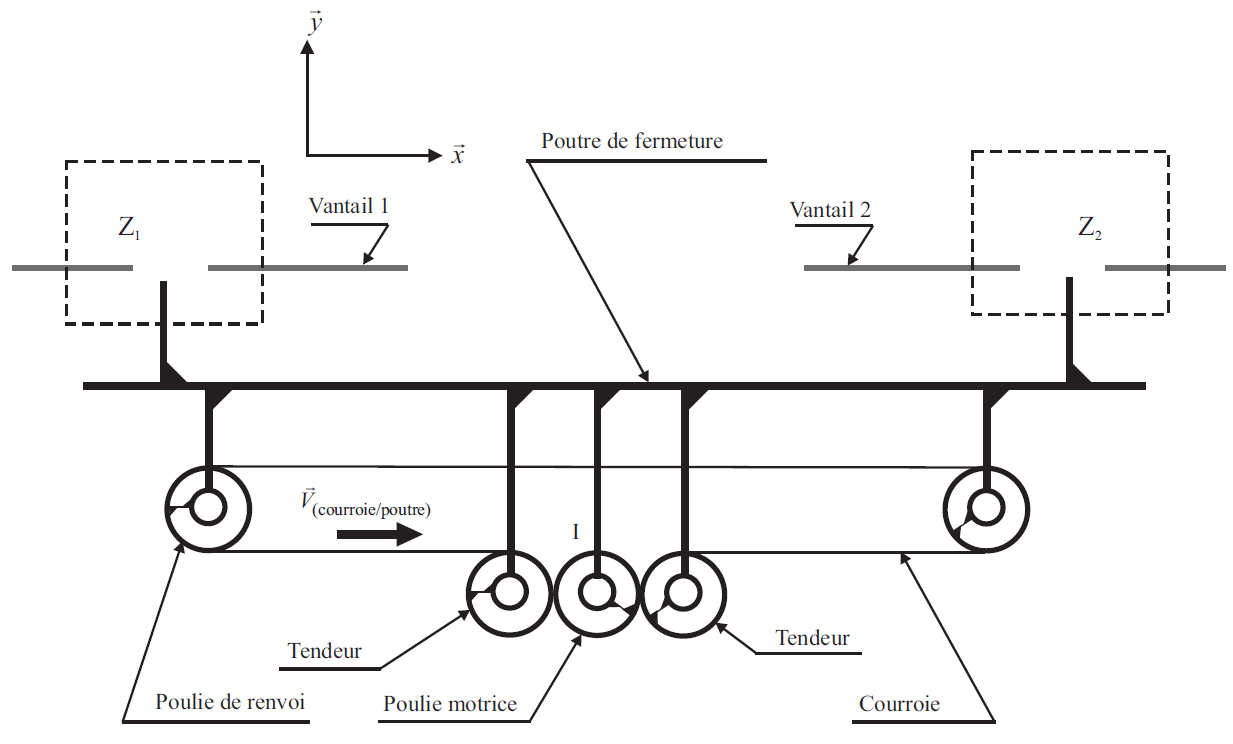
\includegraphics[width=0.8\linewidth]{img/DR2}
\end{center}

\newpage

\reponse{3}{4}

\reponse{4}{5}

\reponse{5}{4}

\newpage

\reponse{6}{0}

\begin{center}
 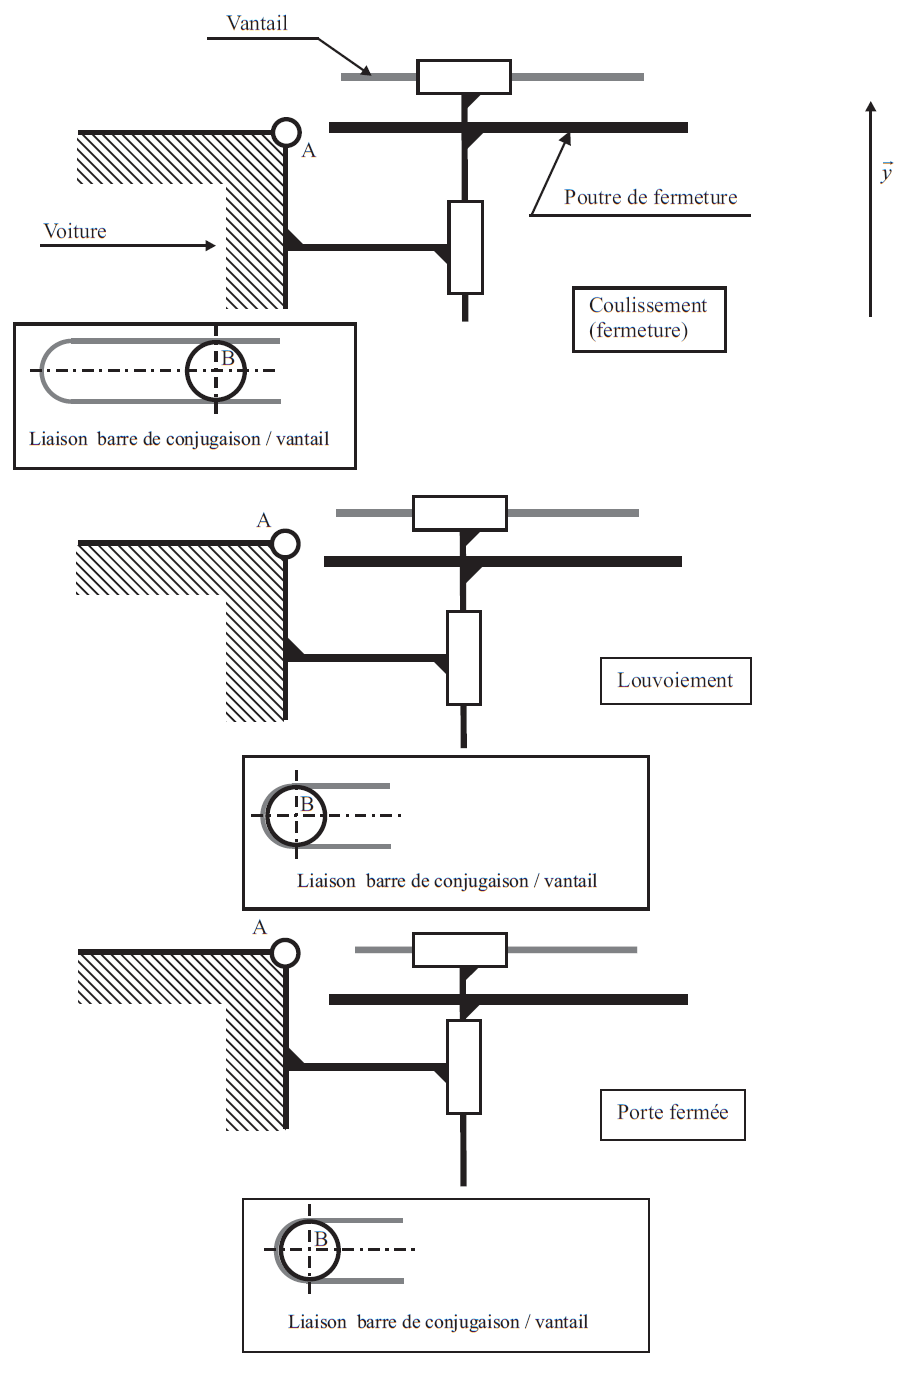
\includegraphics[width=0.8\linewidth]{img/DR3}
\end{center}

\newpage

\reponse{7}{4}

\reponse{8}{4}

\reponse{9}{9}

\reponse{10}{6}

\reponse{11}{5}

\reponse{12}{5}

\newpage

\reponse{13}{5}

\reponse{14}{0}

\begin{center}
 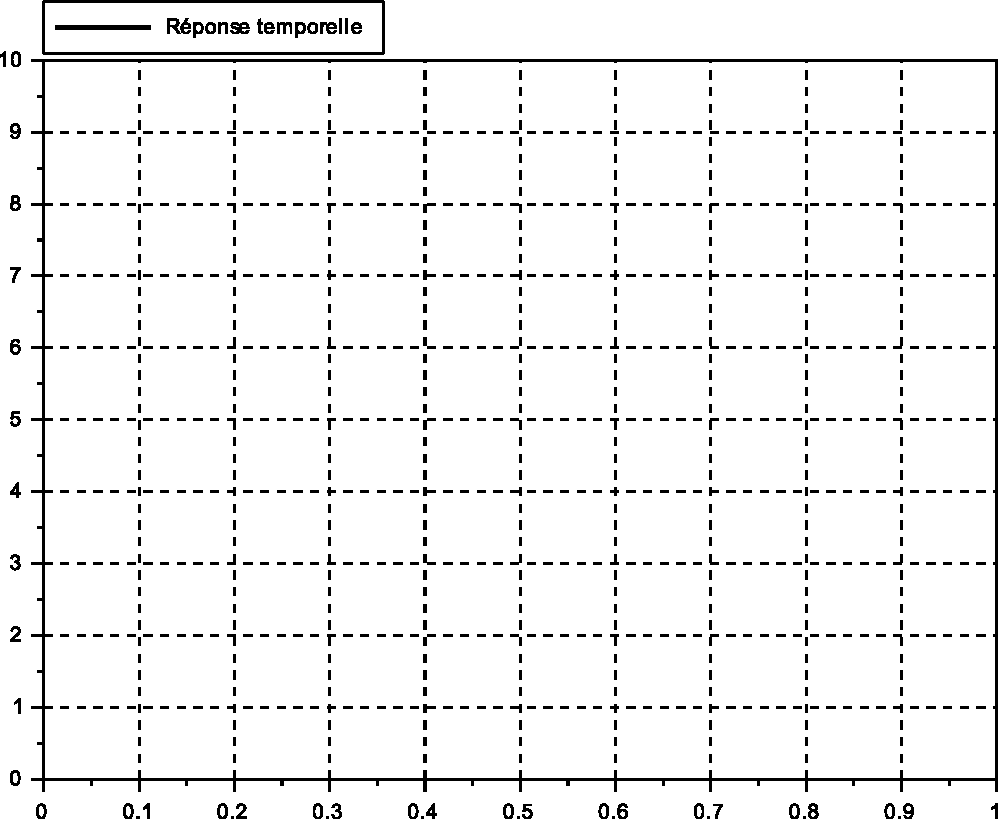
\includegraphics[width=0.8\linewidth]{img/q14}
\end{center}

~\ \\ ~\ \\


\reponse{15}{3}

\reponse{16}{3}

\newpage

\reponse{17}{0}

\begin{center}
 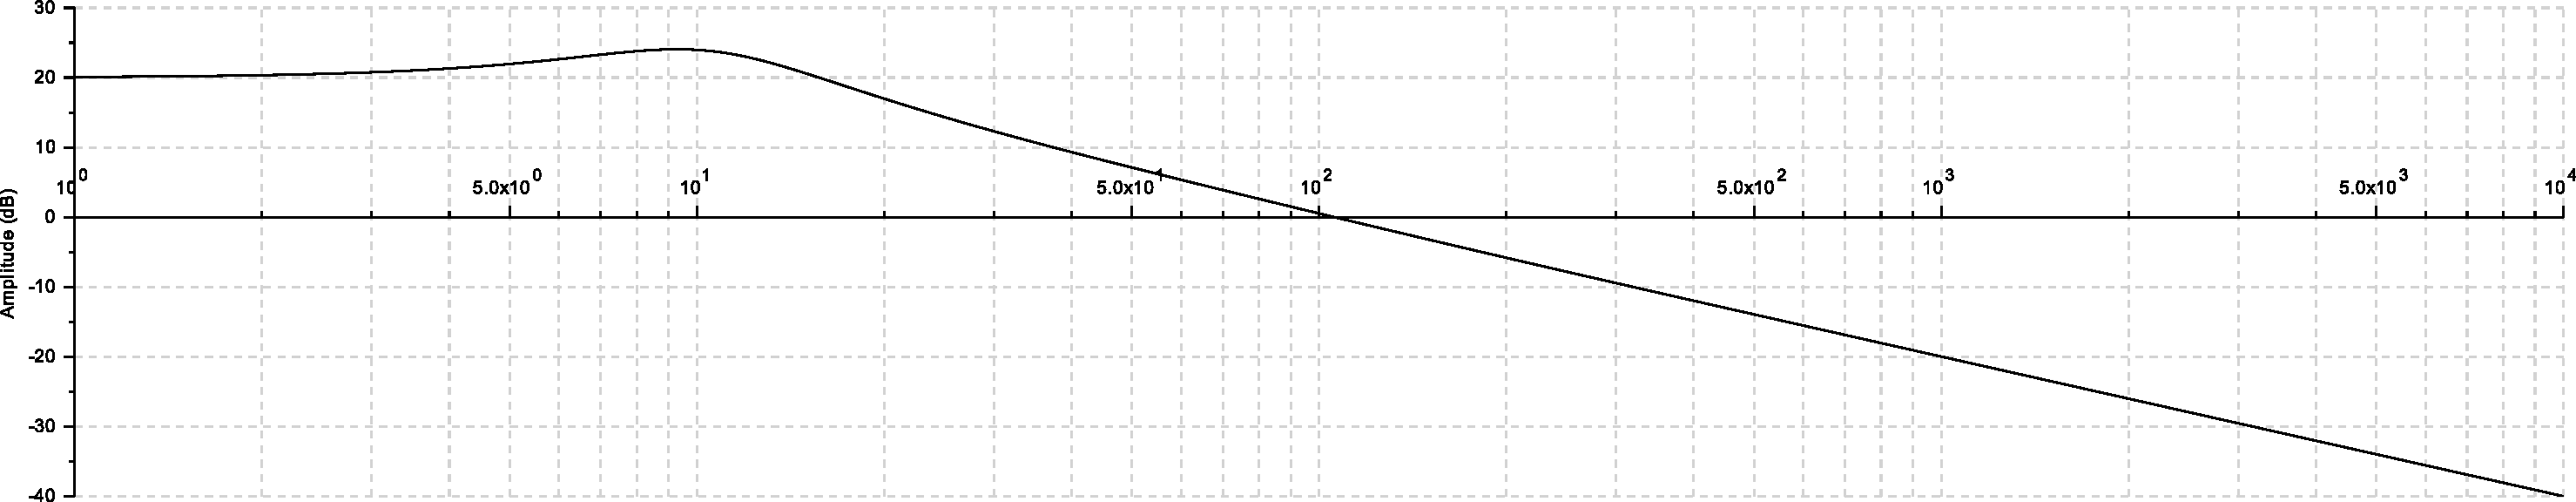
\includegraphics[width=\linewidth]{img/bode}
\end{center}

~\ \\ ~\ \\ ~\ \\ ~\ \\ ~\ \\ ~\ \\ ~\ \\ ~\ \\

\reponse{18}{0}

\begin{center}
 \centering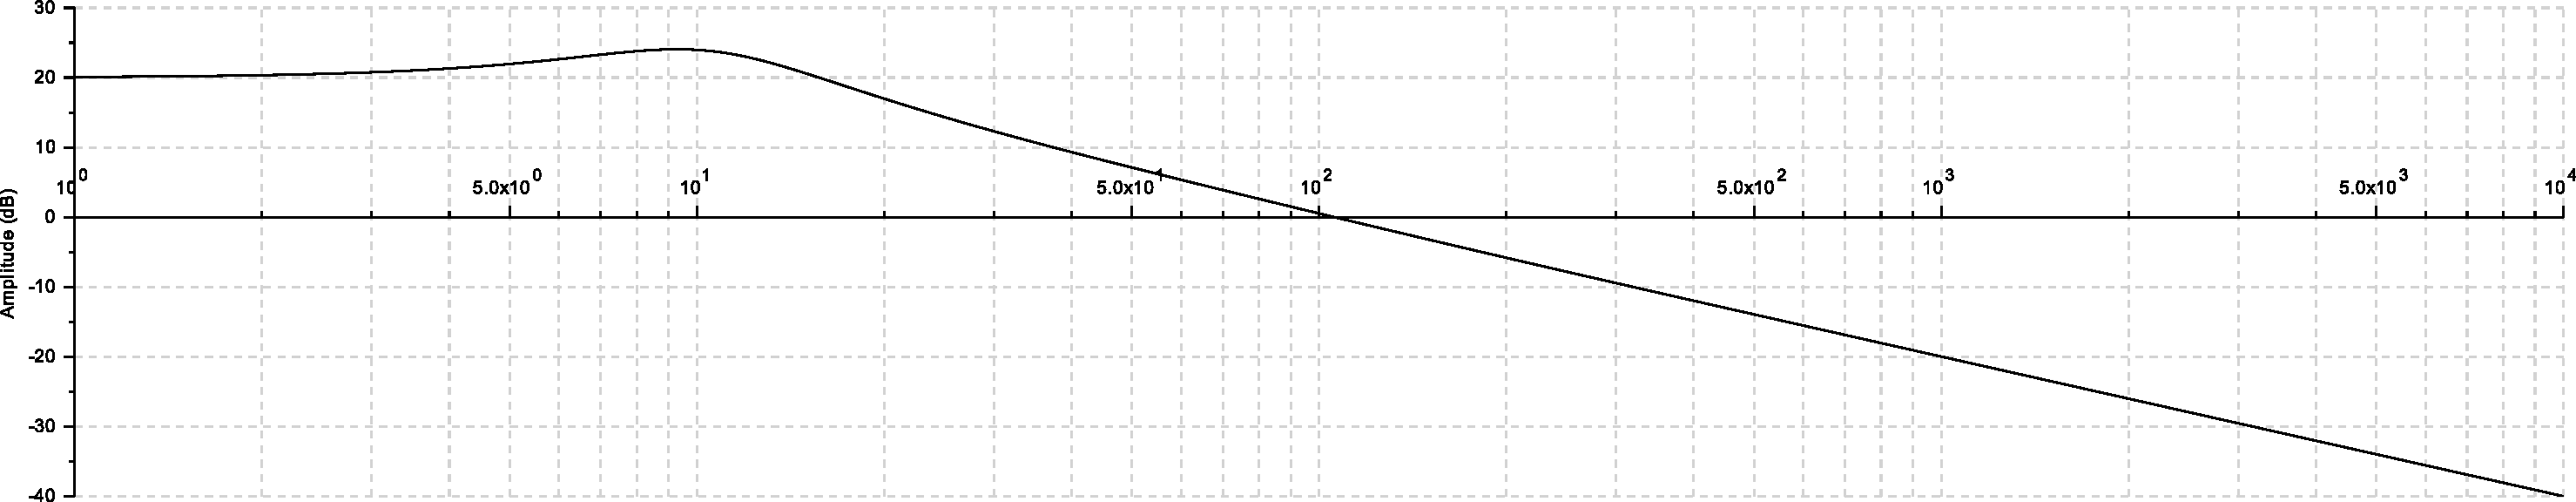
\includegraphics[width=\linewidth]{img/bode}
\end{center}

~\ \\ ~\ \\

\newpage

\reponse{19}{0}

\begin{center}
 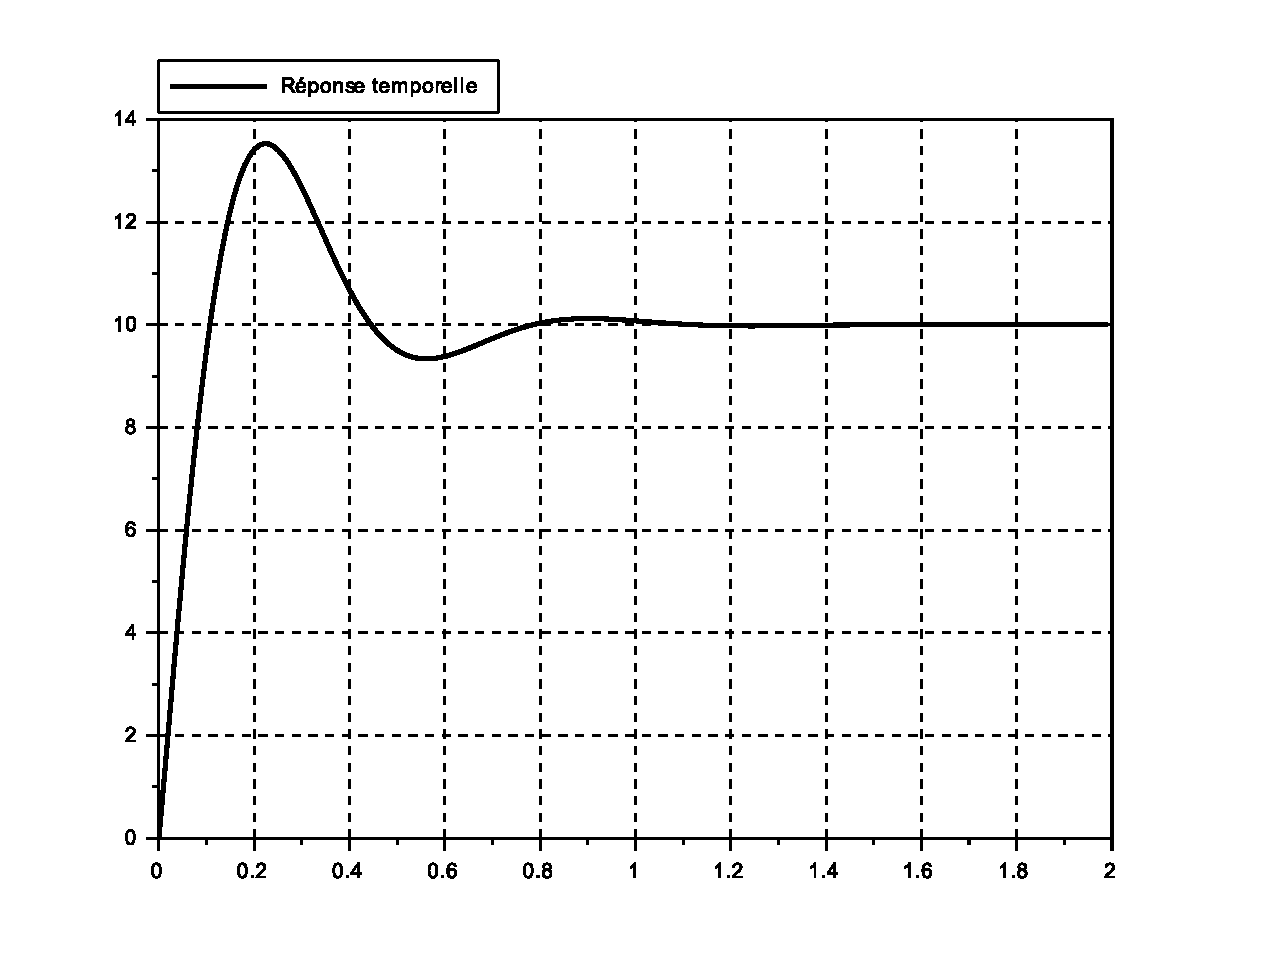
\includegraphics[width=\linewidth]{img/q19}
\end{center}

~\ \\ ~\ \\ ~\ \\ ~\ \\

\reponse{20}{3}

\reponse{21}{3}

\newpage

\reponse{22}{10}

\reponse{23}{0}

\begin{center}
 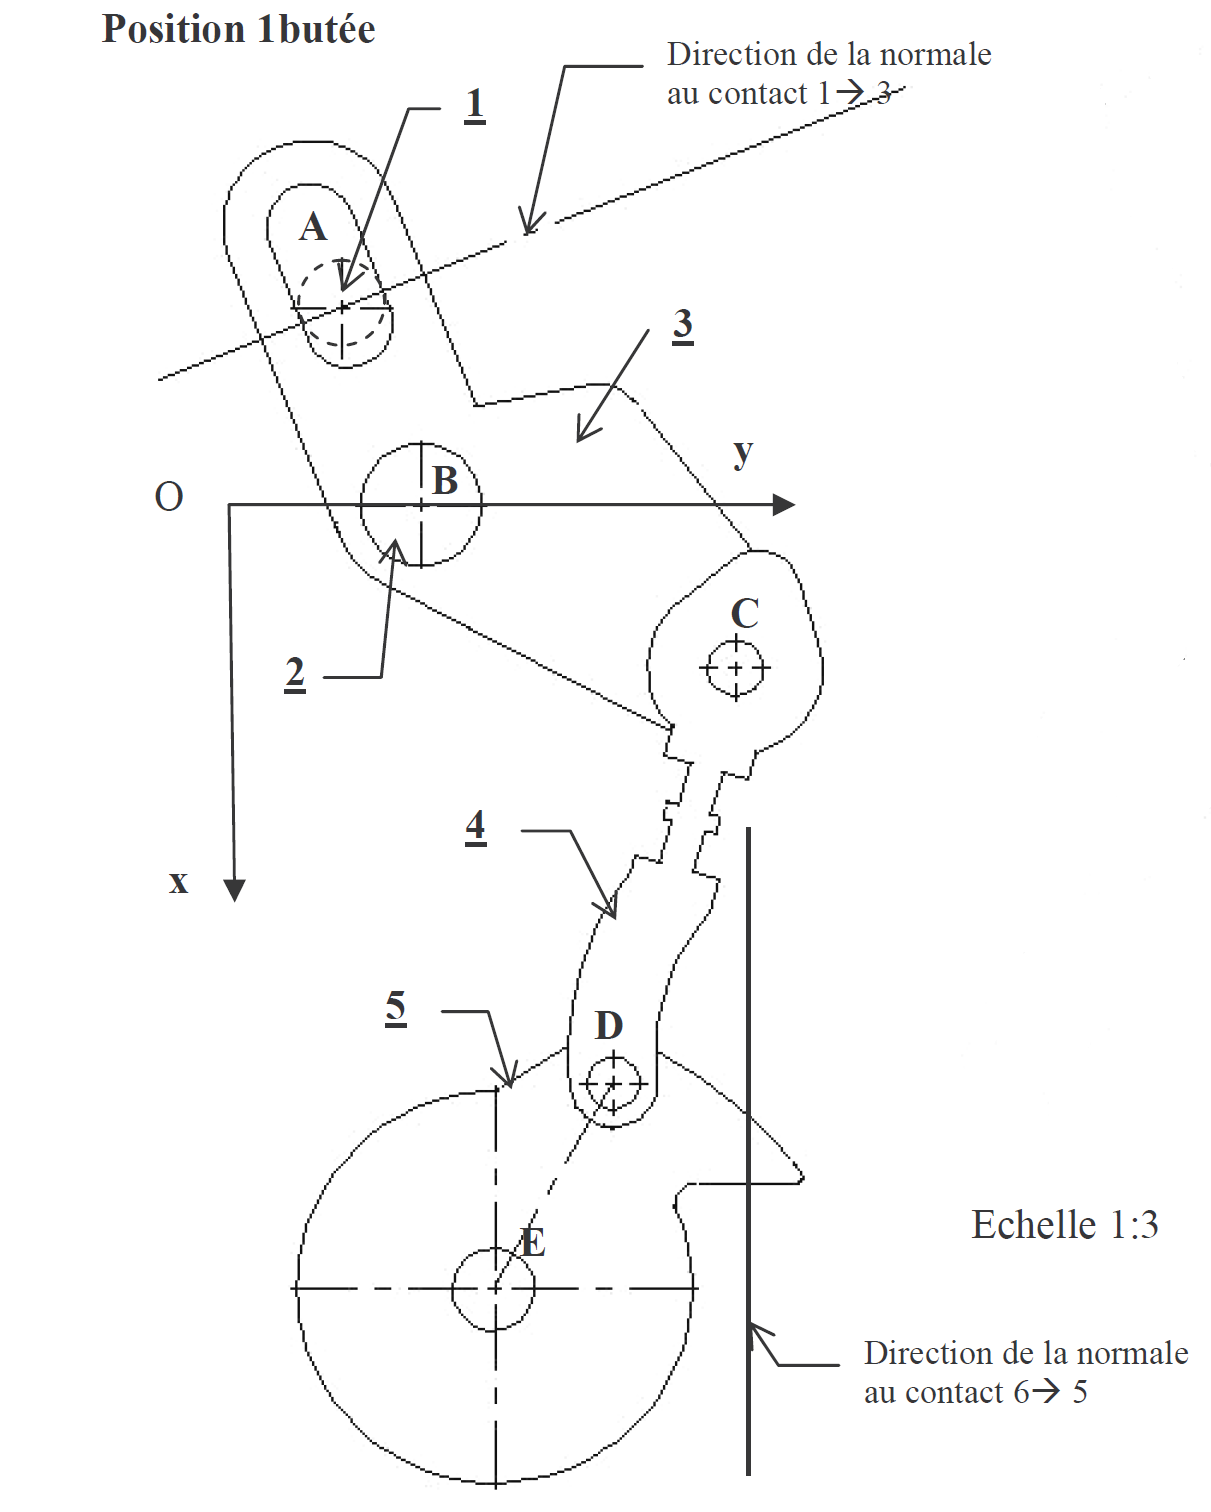
\includegraphics[width=0.7\linewidth]{img/Portes15}
\end{center}

\newpage

\reponse{24}{5}

\reponse{25}{0}

\begin{center}
 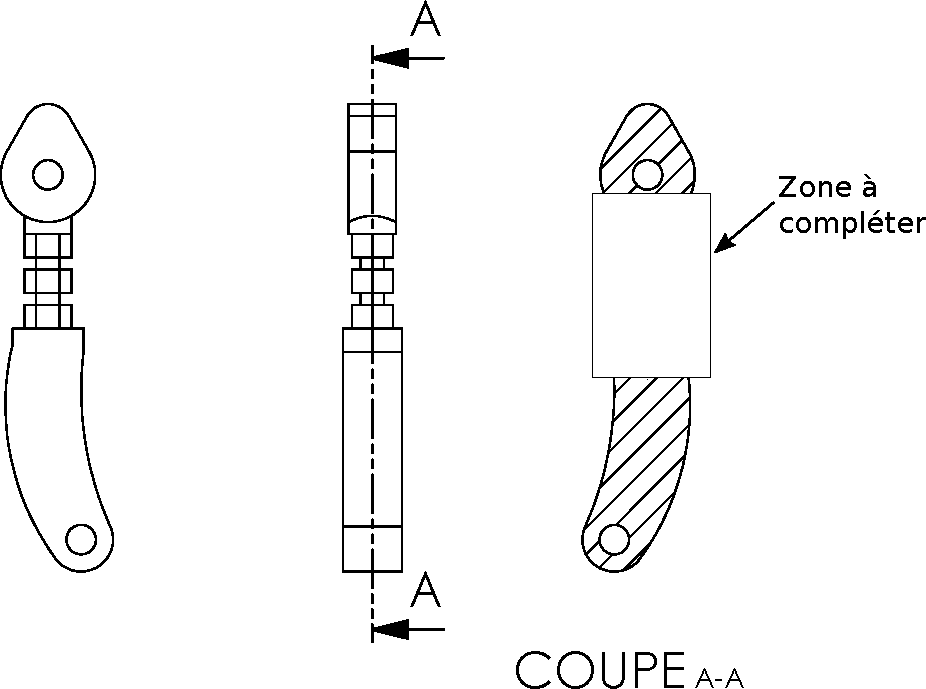
\includegraphics[width=0.8\linewidth]{img/Piece}
\end{center}

\reponse{26}{3}

\ifdef{\public}{\end{document}}{}

\newpage
\cleardoublepage

\pagestyle{correction}

\section{Correction}

\paragraph{Question 1:}

\begin{center}
 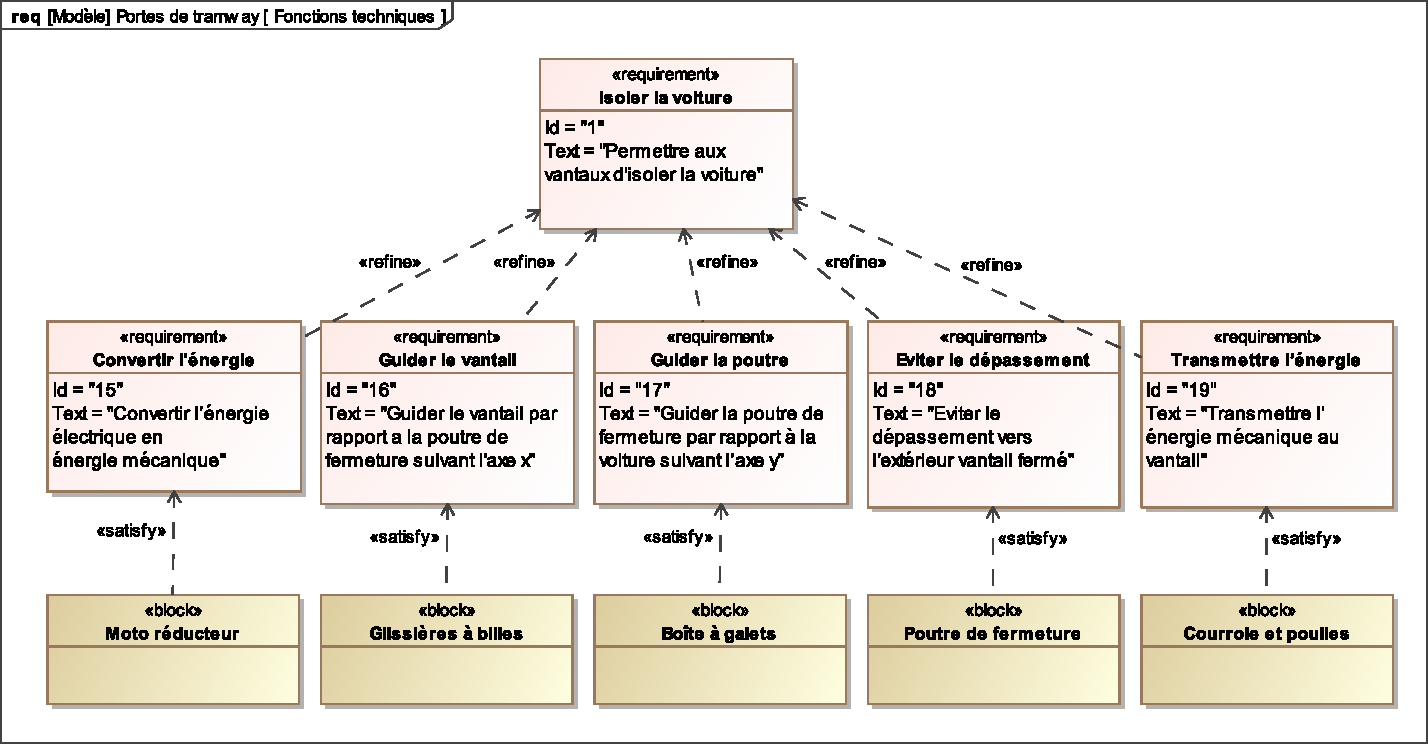
\includegraphics[width=\linewidth]{img/fonctions_techniques_cor}
\end{center}

\subsection{Étude partielle de la phase de fermeture}

\paragraph{Question 2:}

\begin{center}
 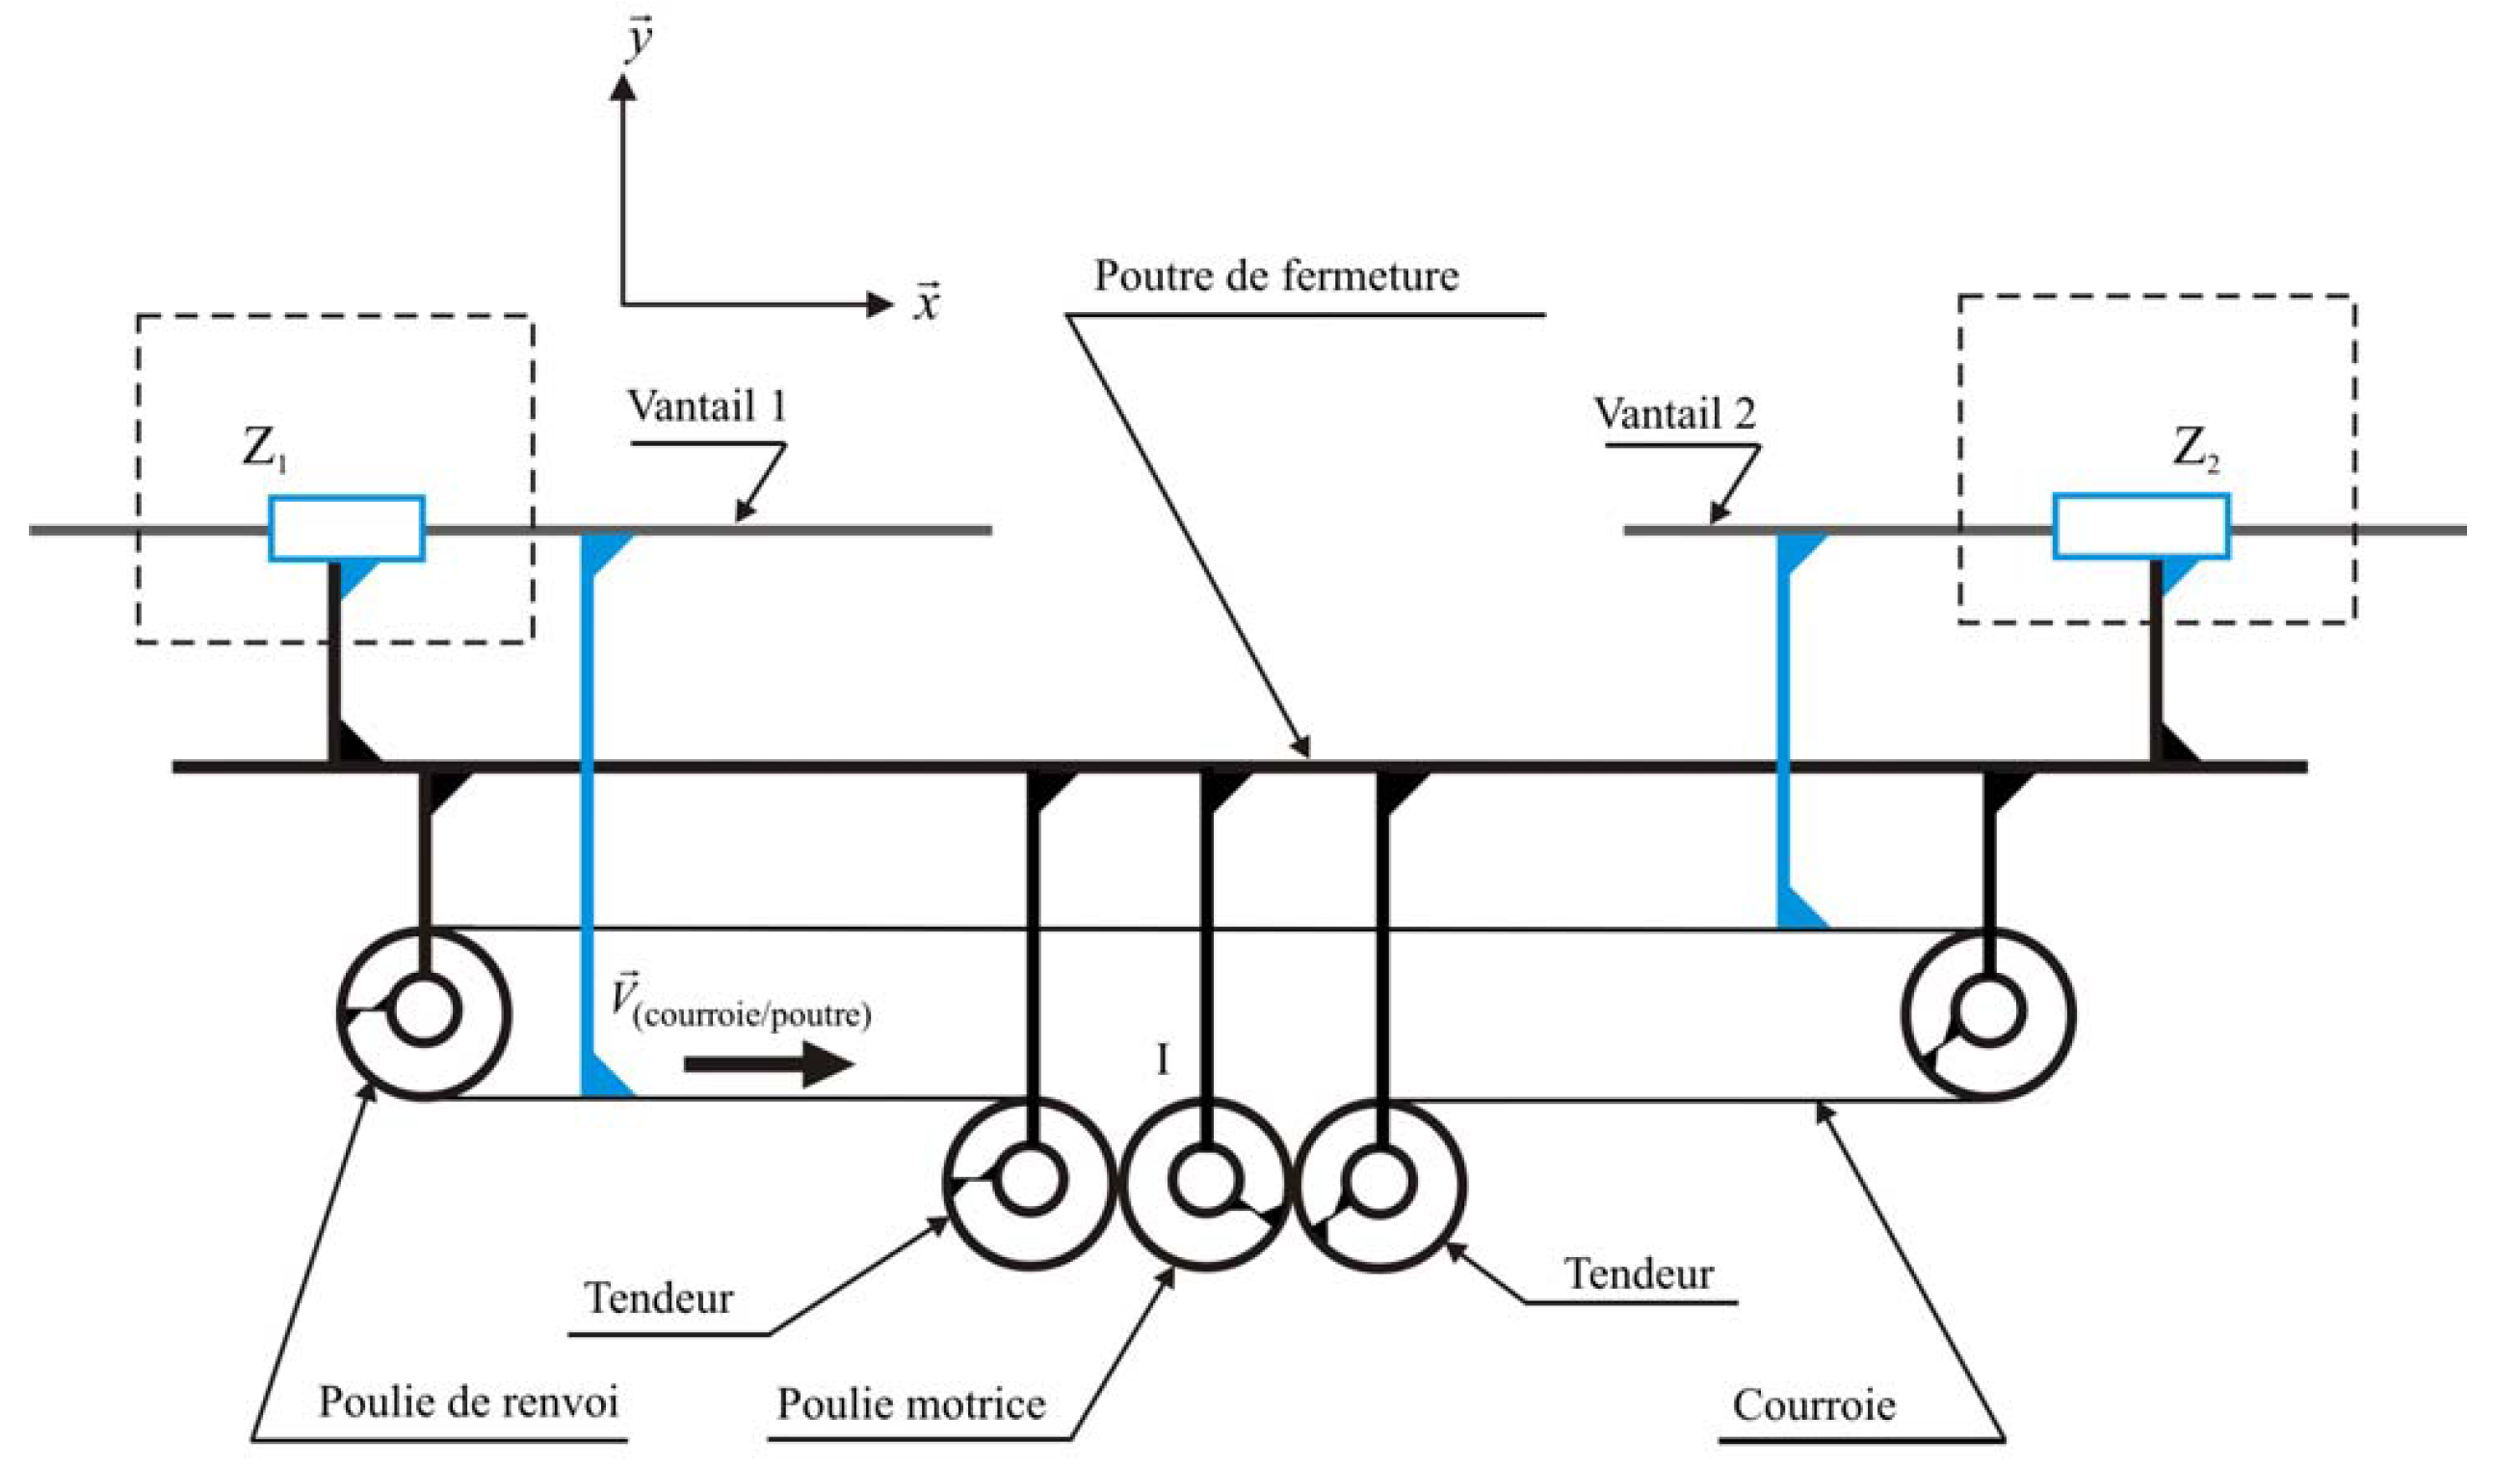
\includegraphics[width=\linewidth]{img/DR2_cor}
\end{center}

\paragraph{Question 3:}

$rs=6.(p-1)-m=6.(2-1)-1=5$
$Ns=2.4=8$

$h=Ns-rs=8-5=3$.

\paragraph{Question 4:}

$\left\{V_{p/v}\right\}=\left\{
\begin{matrix}
 0 & 0 \\
 0 & Vy_{H,pv} \\
 0 & 0 
\end{matrix}
\right \}_{H,R}=\left \{
\begin{matrix}
 \overrightarrow{0} \\ 
 V_{H,p/v}.\overrightarrow{y} 
\end{matrix}
\right\}_H$


\paragraph{Question 5:}

Liaison ponctuelle:

$\left\{V^1_{p/v}\right\}=\left\{
\begin{matrix}
 \omega x_{pv1} & Vx_{H,pv1} \\
 \omega y_{pv1} & Vy_{H,pv1} \\
 \omega z_{pv1} & 0 
\end{matrix}
\right \}_{J,R}$

$\left\{V^2_{p/v}\right\}=\left\{
\begin{matrix}
 0 & 0 \\
 \omega y_{pv2} & Vy_{H,pv2} \\
 0 & 0 
\end{matrix}
\right \}_{H,R}=\left\{
\begin{matrix}
 0 & 0 \\
 \omega y_{pv2} & Vy_{H,pv2} \\
 0 & -l_3.\omega y_{pv2}
\end{matrix}
\right \}_{J,R}$

Donc, 
$\left\{V^1_{p/v}\right\}=\left\{
\begin{matrix}
 \omega x_{pv1} & Vx_{H,pv1} \\
 \omega y_{pv1} & Vy_{H,pv1} \\
 \omega z_{pv1} & 0 
\end{matrix}
\right \}_{J,R}=\left\{
\begin{matrix}
 0 & 0 \\
 \omega y_{pv2} & Vy_{H,pv2} \\
 0 & -l_3.\omega y_{pv2}
\end{matrix}
\right \}_{J,R}$

La liaison équivalente est bien une glissière et h=0.

\newpage

\paragraph{Question 6:}

\begin{center}
 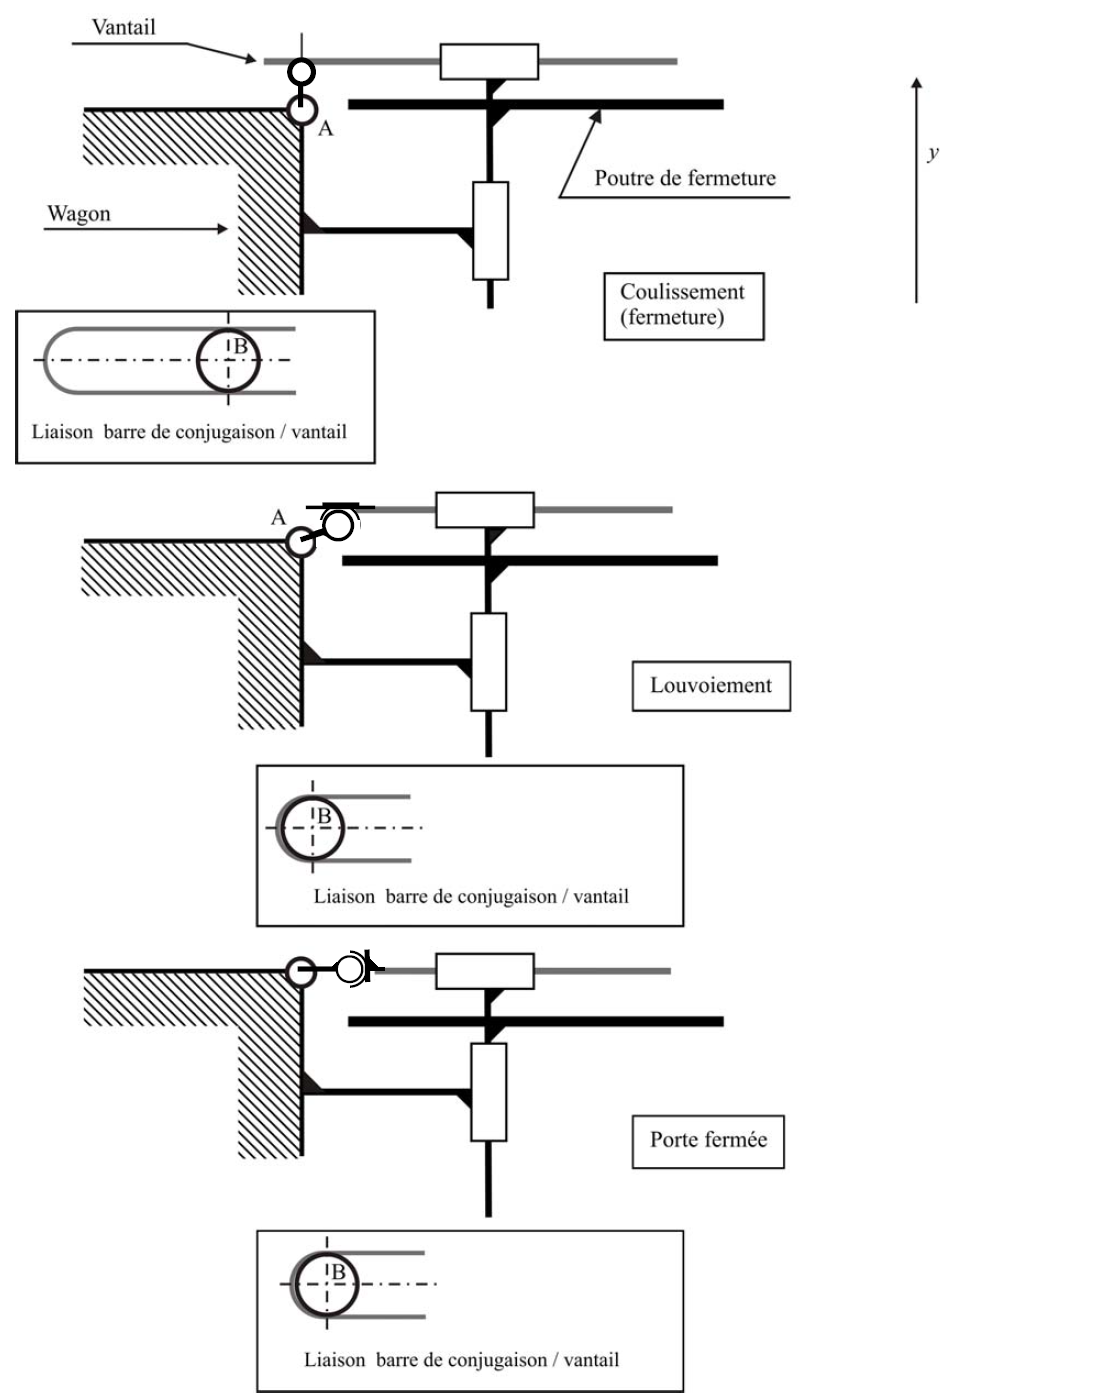
\includegraphics[width=\linewidth]{img/DR3_cor}
\end{center}

\newpage

\subsection{Étude de la phase de verrouillage}

\paragraph{Question 7:}

$x(t)=l_1.cos\theta(t)+l_2.\sqrt{1-\left(\frac{l_1}{l_2}\right)^2.sin^2\theta(t)}$

\paragraph{Question 8:}

$\left\{V_{4/1}\right\}=\left\{V_{4/3}\right\}+\left\{V_{3/2}\right\}+\left\{V_{2/1}\right\}$

\paragraph{Question 9:}

$\left\{V_{4/1}\right\}=\left\{
\begin{matrix}
\omega x_{41} & Vx_{E,41} \\
0 & 0 \\
0 & 0 
\end{matrix}
\right \}_{E,R}$

$\left\{V_{4/3}\right\}=\left\{
\begin{matrix}
0 & 0 \\
0 & 0 \\
\omega z_{43} & 0 
\end{matrix}
\right \}_{E,R}$

$\left\{V_{3/2}\right\}=\left\{
\begin{matrix}
0 & 0 \\
0 & 0 \\
\omega z_{32} & 0 
\end{matrix}
\right \}_{F,R}$

$\left\{V_{2/1}\right\}=\left\{
\begin{matrix}
0 & 0 \\
0 & 0 \\
\omega z_{21} & 0 
\end{matrix}
\right \}_{I,R}$

\paragraph{Question 10:}

$Vx_{E,40}=\frac{l_1.sin\theta(t).x(t)}{l_1.cos\theta(t)-x(t)}.\omega z_{21}$


\subsection{Étude de la commande de la chaîne de motorisation}

\paragraph{Question 11:}

$H(p)=\frac{10.(1+0,01.p)}{1+\frac{1}{10.K_r}.p+\frac{0,01}{10.K_r}.p^2}$

$H(p)=\frac{10.(1+0,01.p)}{1+0,1.p+0,001.p^2}$

\paragraph{Question 12:}

Les autres coefficients étant négligeables devant ceux qui restent,

$H(p)=\frac{10}{1+0,1.p}$

\paragraph{Question 13:}

$\omega_1(t)=10(1-e^{-10.t})$

\newpage

\paragraph{Question 14:}

\begin{center}
 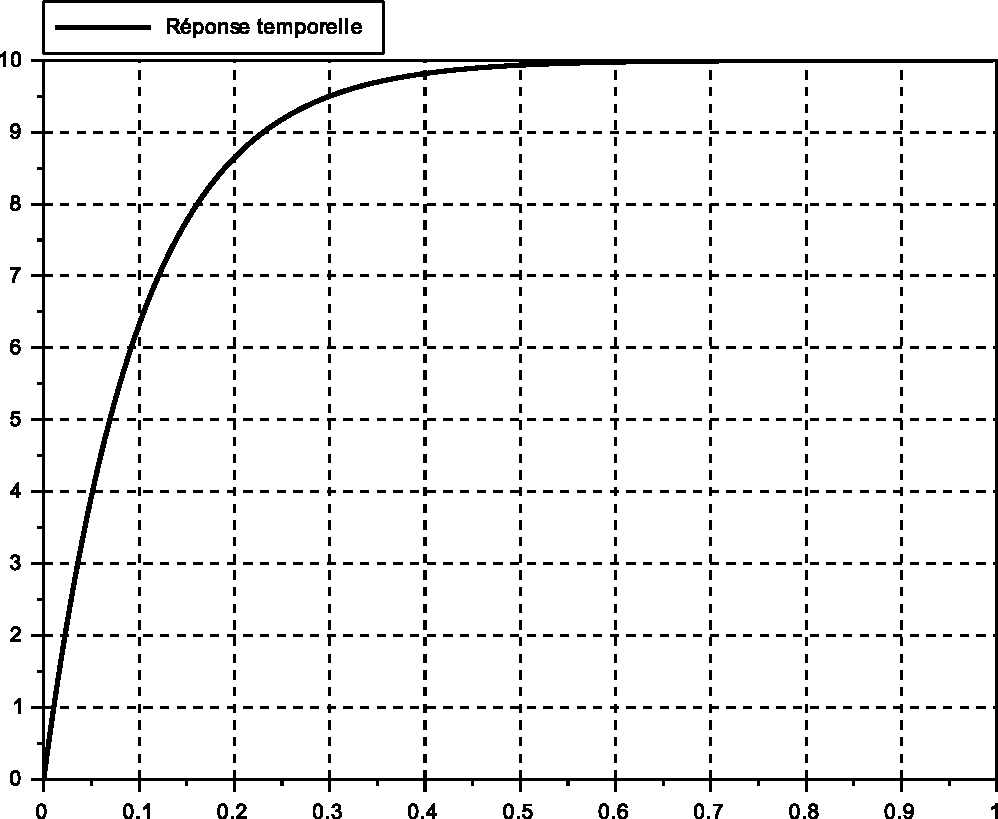
\includegraphics[width=0.8\linewidth]{img/q14_cor}
\end{center}

\paragraph{Question 15:}

$t_{R,5\%}=3.\tau=0,3s$

\paragraph{Question 16:}

$H(p)=10.\frac{1+0,11.p+0,001.p^2}{1+0,1.p+0,01.p^2+0,0001.p^3}$

C'est une fonction de classe 0 et d'ordre 3.

\paragraph{Question 17:}

\begin{center}
 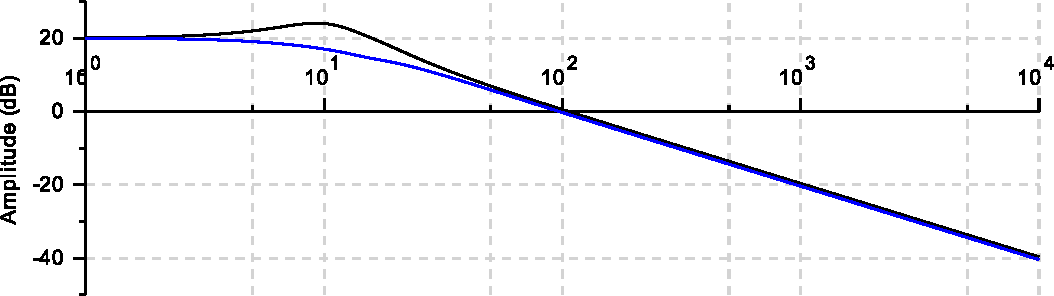
\includegraphics[width=\linewidth]{img/q17_cor}
\end{center}

$H_{ordre1}(p)=\frac{10}{1+0,1.p}$.

$K_{ordre1}=10$ et $\tau_{ordre1}=0,1s$.

\newpage

\paragraph{Question 18:}

\begin{center}
 \centering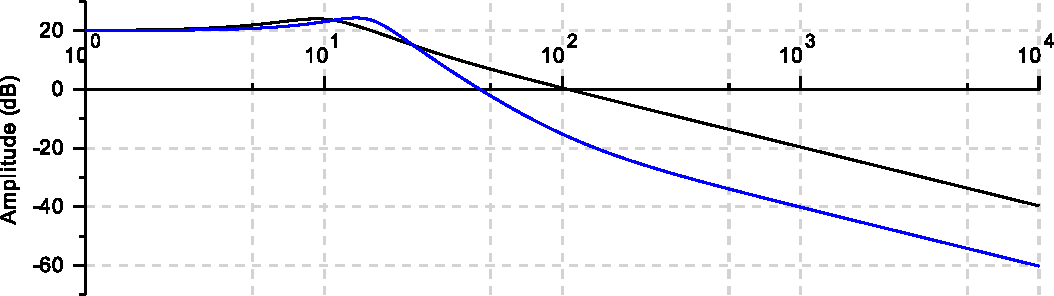
\includegraphics[width=\linewidth]{img/q18_cor}
\end{center}

$20.log\left(\frac{1}{2.z.\sqrt{1-z^2}}\right)=4$

$H_{ordre2}(p)=\frac{10}{1+2.\frac{0,32}{15}.p+(\frac{p}{15})^2}$.

$K_{ordre2}=10$, $\xi_{ordre2}=0,32$ et $\omega0_{ordre2}=15rad.s^{-1}$, 

\paragraph{Question 19:}

\begin{center}
 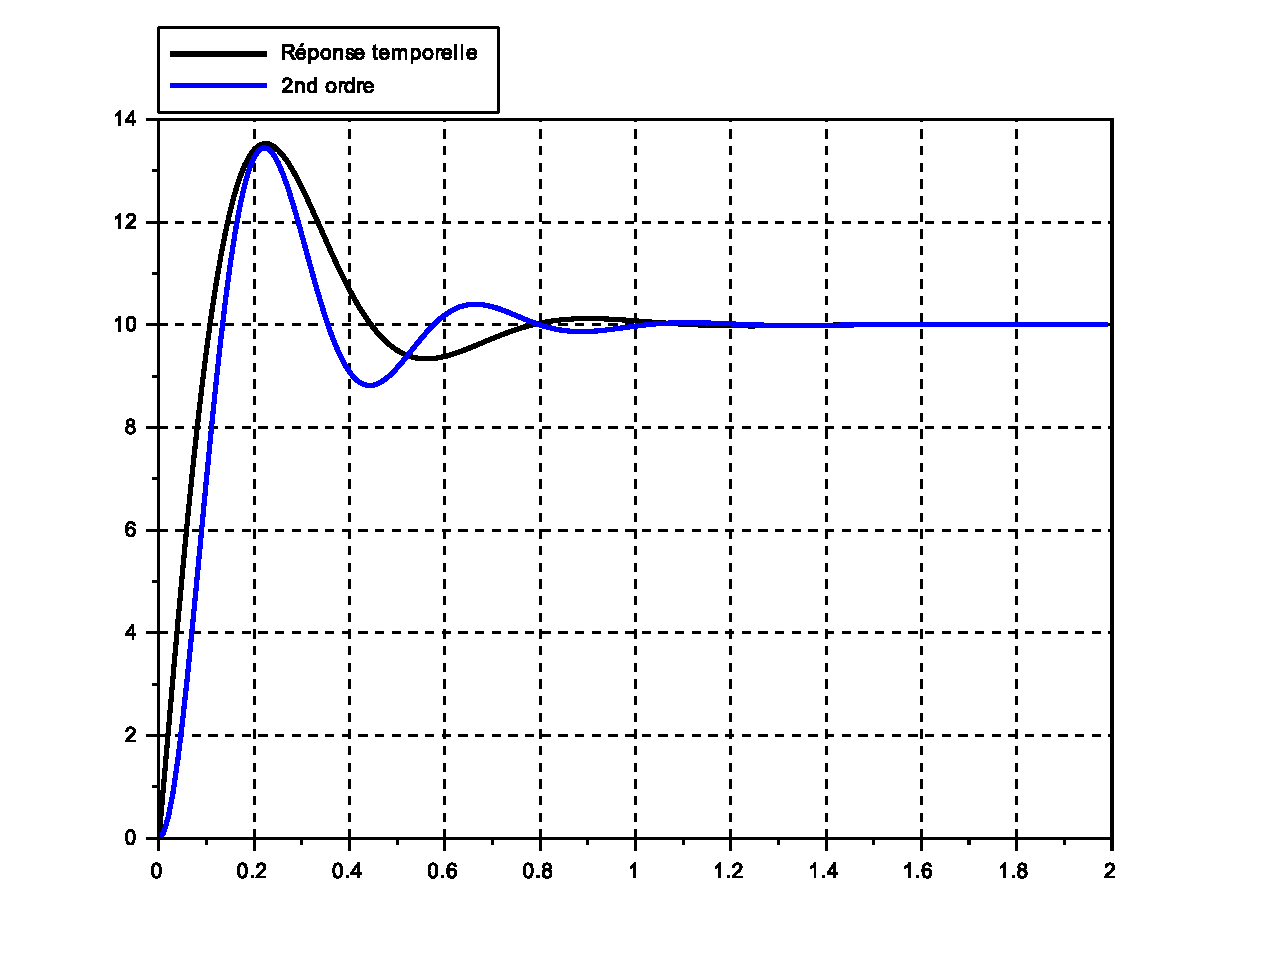
\includegraphics[width=\linewidth]{img/q19_cor}
\end{center}

On retrouve la fonction précédente, donc:

$K_{ordre2}=10$, $\xi_{ordre2}=0,32$ et $\omega0_{ordre2}=15rad.s^{-1}$.

\paragraph{Question 20:}

D'après la lecture sur le graphique, $t_{R,5\%}=0,6s$.

\paragraph{Question 21:}

Cette correction n'a pas permis d'améliorer le temps de réponse.

\subsection{Étude du système de verrouillage de la porte}

\paragraph{Question 22:}

\begin{center}
 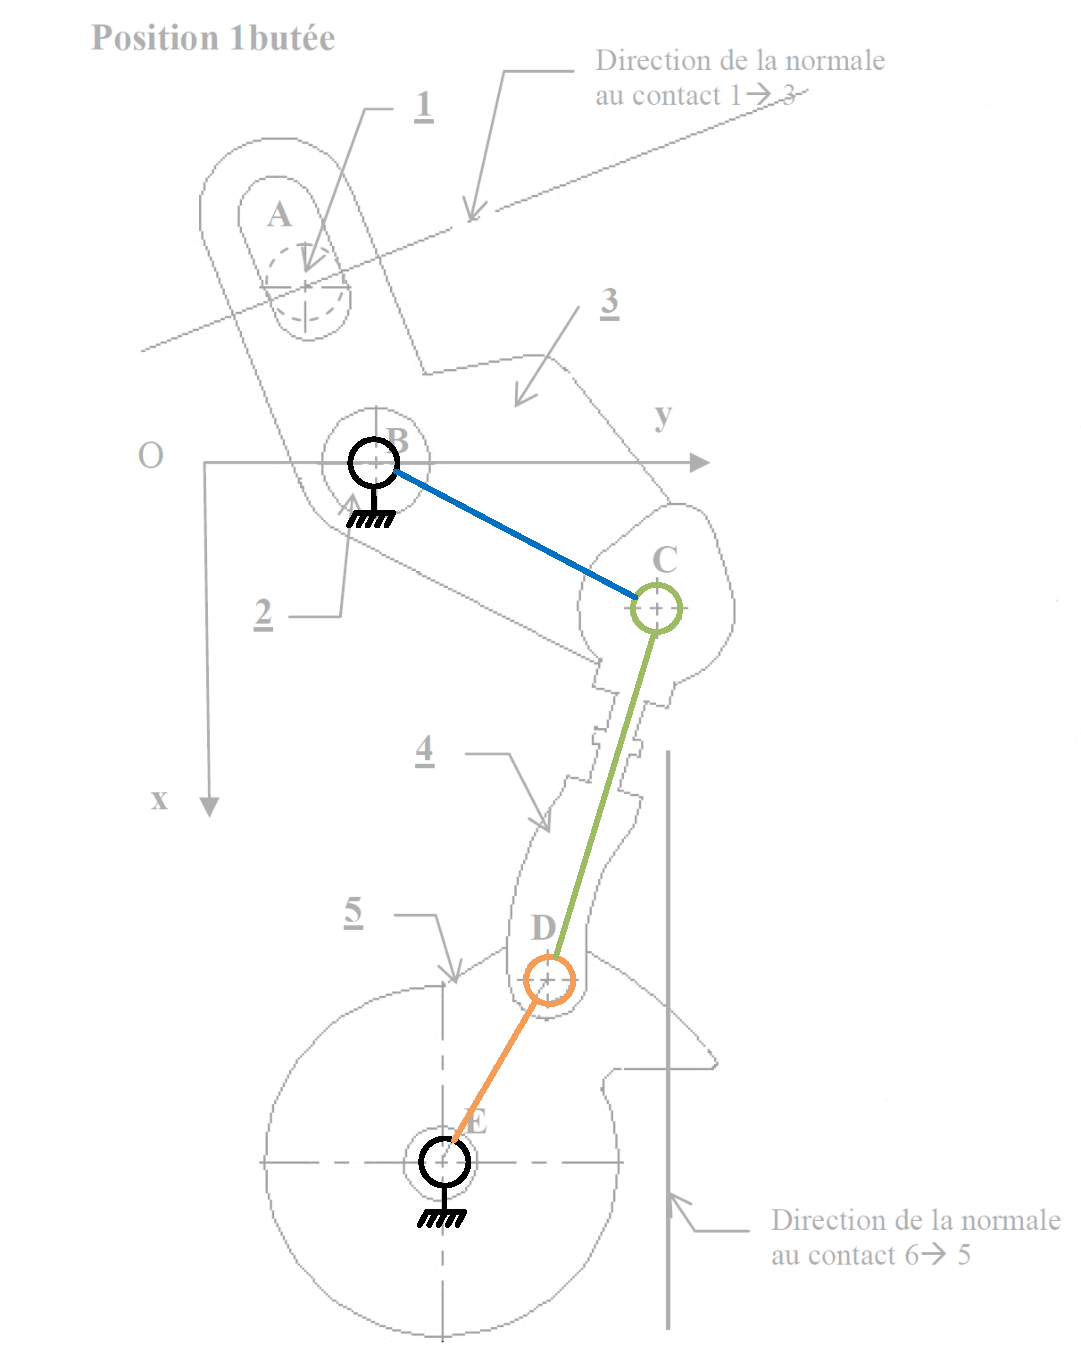
\includegraphics[width=0.7\linewidth]{img/cin}
\end{center}

\newpage

\paragraph{Question 23:}

\begin{center}
 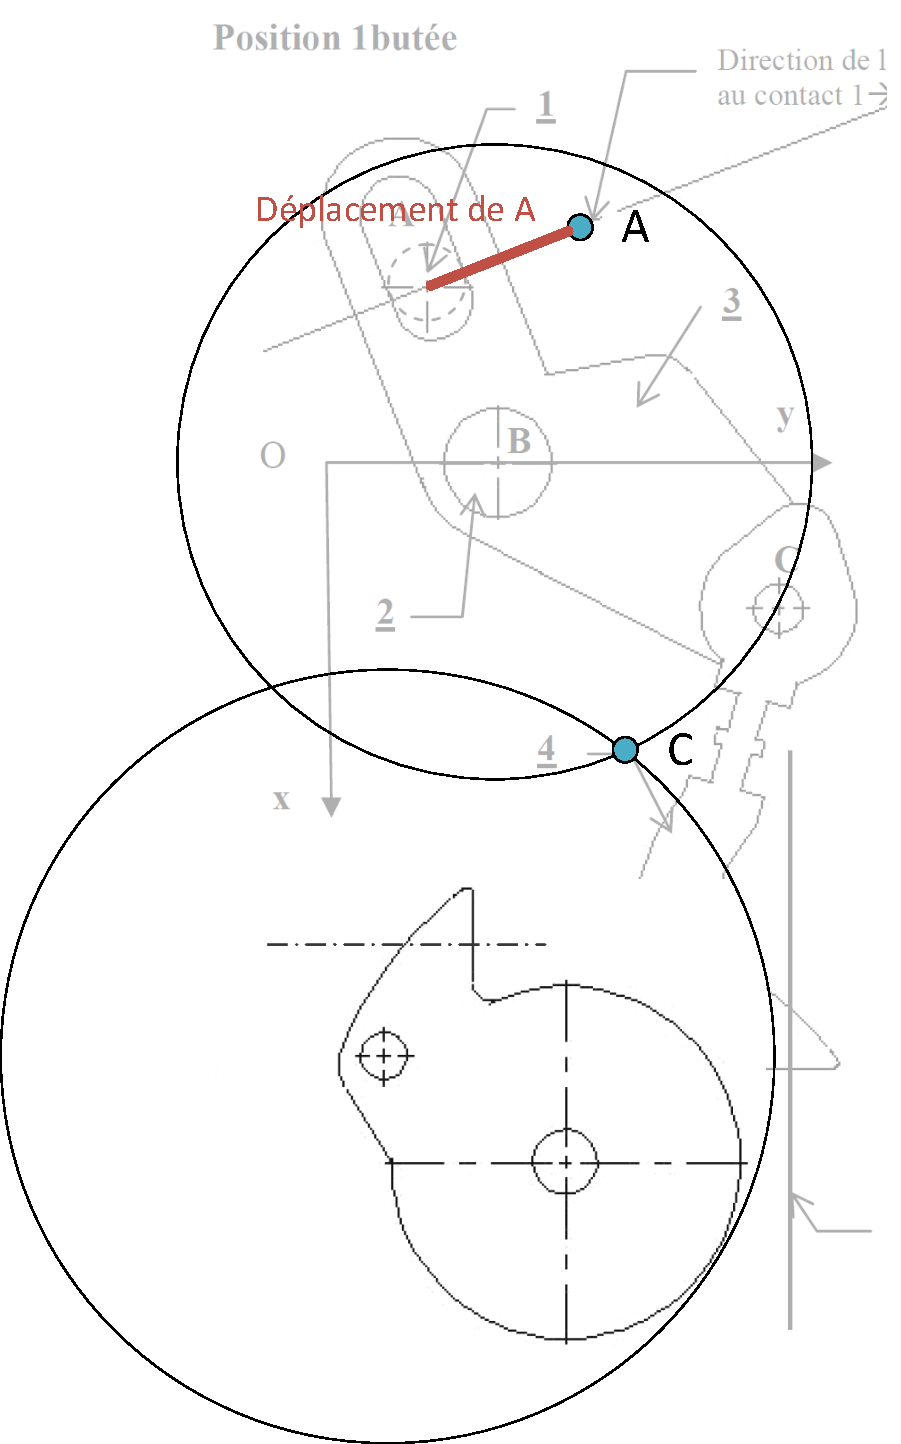
\includegraphics[width=0.7\linewidth]{img/geometrie}
\end{center}

\paragraph{Question 24:}

La distance à parcourir est de 20mm à l'échelle 1:3, donc 60mm.

\newpage

\paragraph{Question 25:}

\begin{center}
 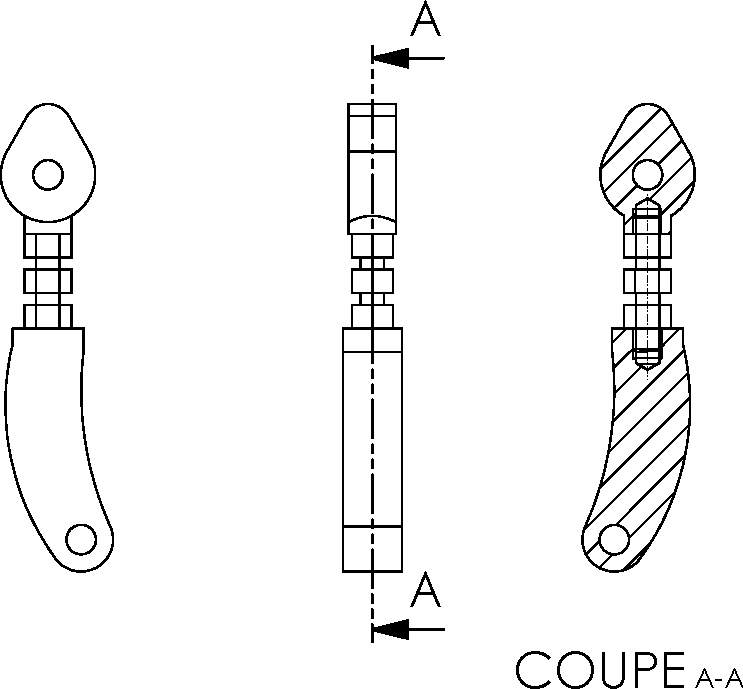
\includegraphics[width=0.6\linewidth]{img/Piece_cor}
\end{center}


\paragraph{Question 26:}

Il faut que les deux pas de vis soient de sens opposés pour que le système fonctionne.

\end{document}
